\documentclass[../thesis.tex]{subfiles}
% Separate preamble for this subfile. This preamble is loaded last, so one can override various functions before \begin{document}

% Better comment extension for Vscode colors these comments differently
% Normal comment color
% * Important information
% ! ALERT
% ? Question
% TODO stuff to do
% // This is strikethrough


\begin{document}

Informally, to tile refers to the process of covering some surface with objects. These objects are called tiles and come in a variety of shapes and sizes. When we are tiling, we essentially place copies of the tile next to each other in a systematic way, intending to leave no gaps and no overlaps between the tiles \cite{kolountzakisTilingsTranslation2010}. The resulting tiling can be as simple as the one shown in \cref{fig:tiling_one} where we have used a single tile, the unit square, to tile the plane, or as complex as \cref{fig:tiling_two} where we have used four different tiles to tile the plane. The first is an example of what is known as a \emph{monohedral tiling} in which all tiles are congruent, and the latter is an example of a Penrose tiling which are well known for being non-periodic \cite[p. 20, 531]{grunbaumTilingsPatterns1987}. %* 1979 page 535 har også penrose tilings




\begin{figure}[h!]%h!
    \centering
    \begin{subfigure}{.47\textwidth}
        \centering
        %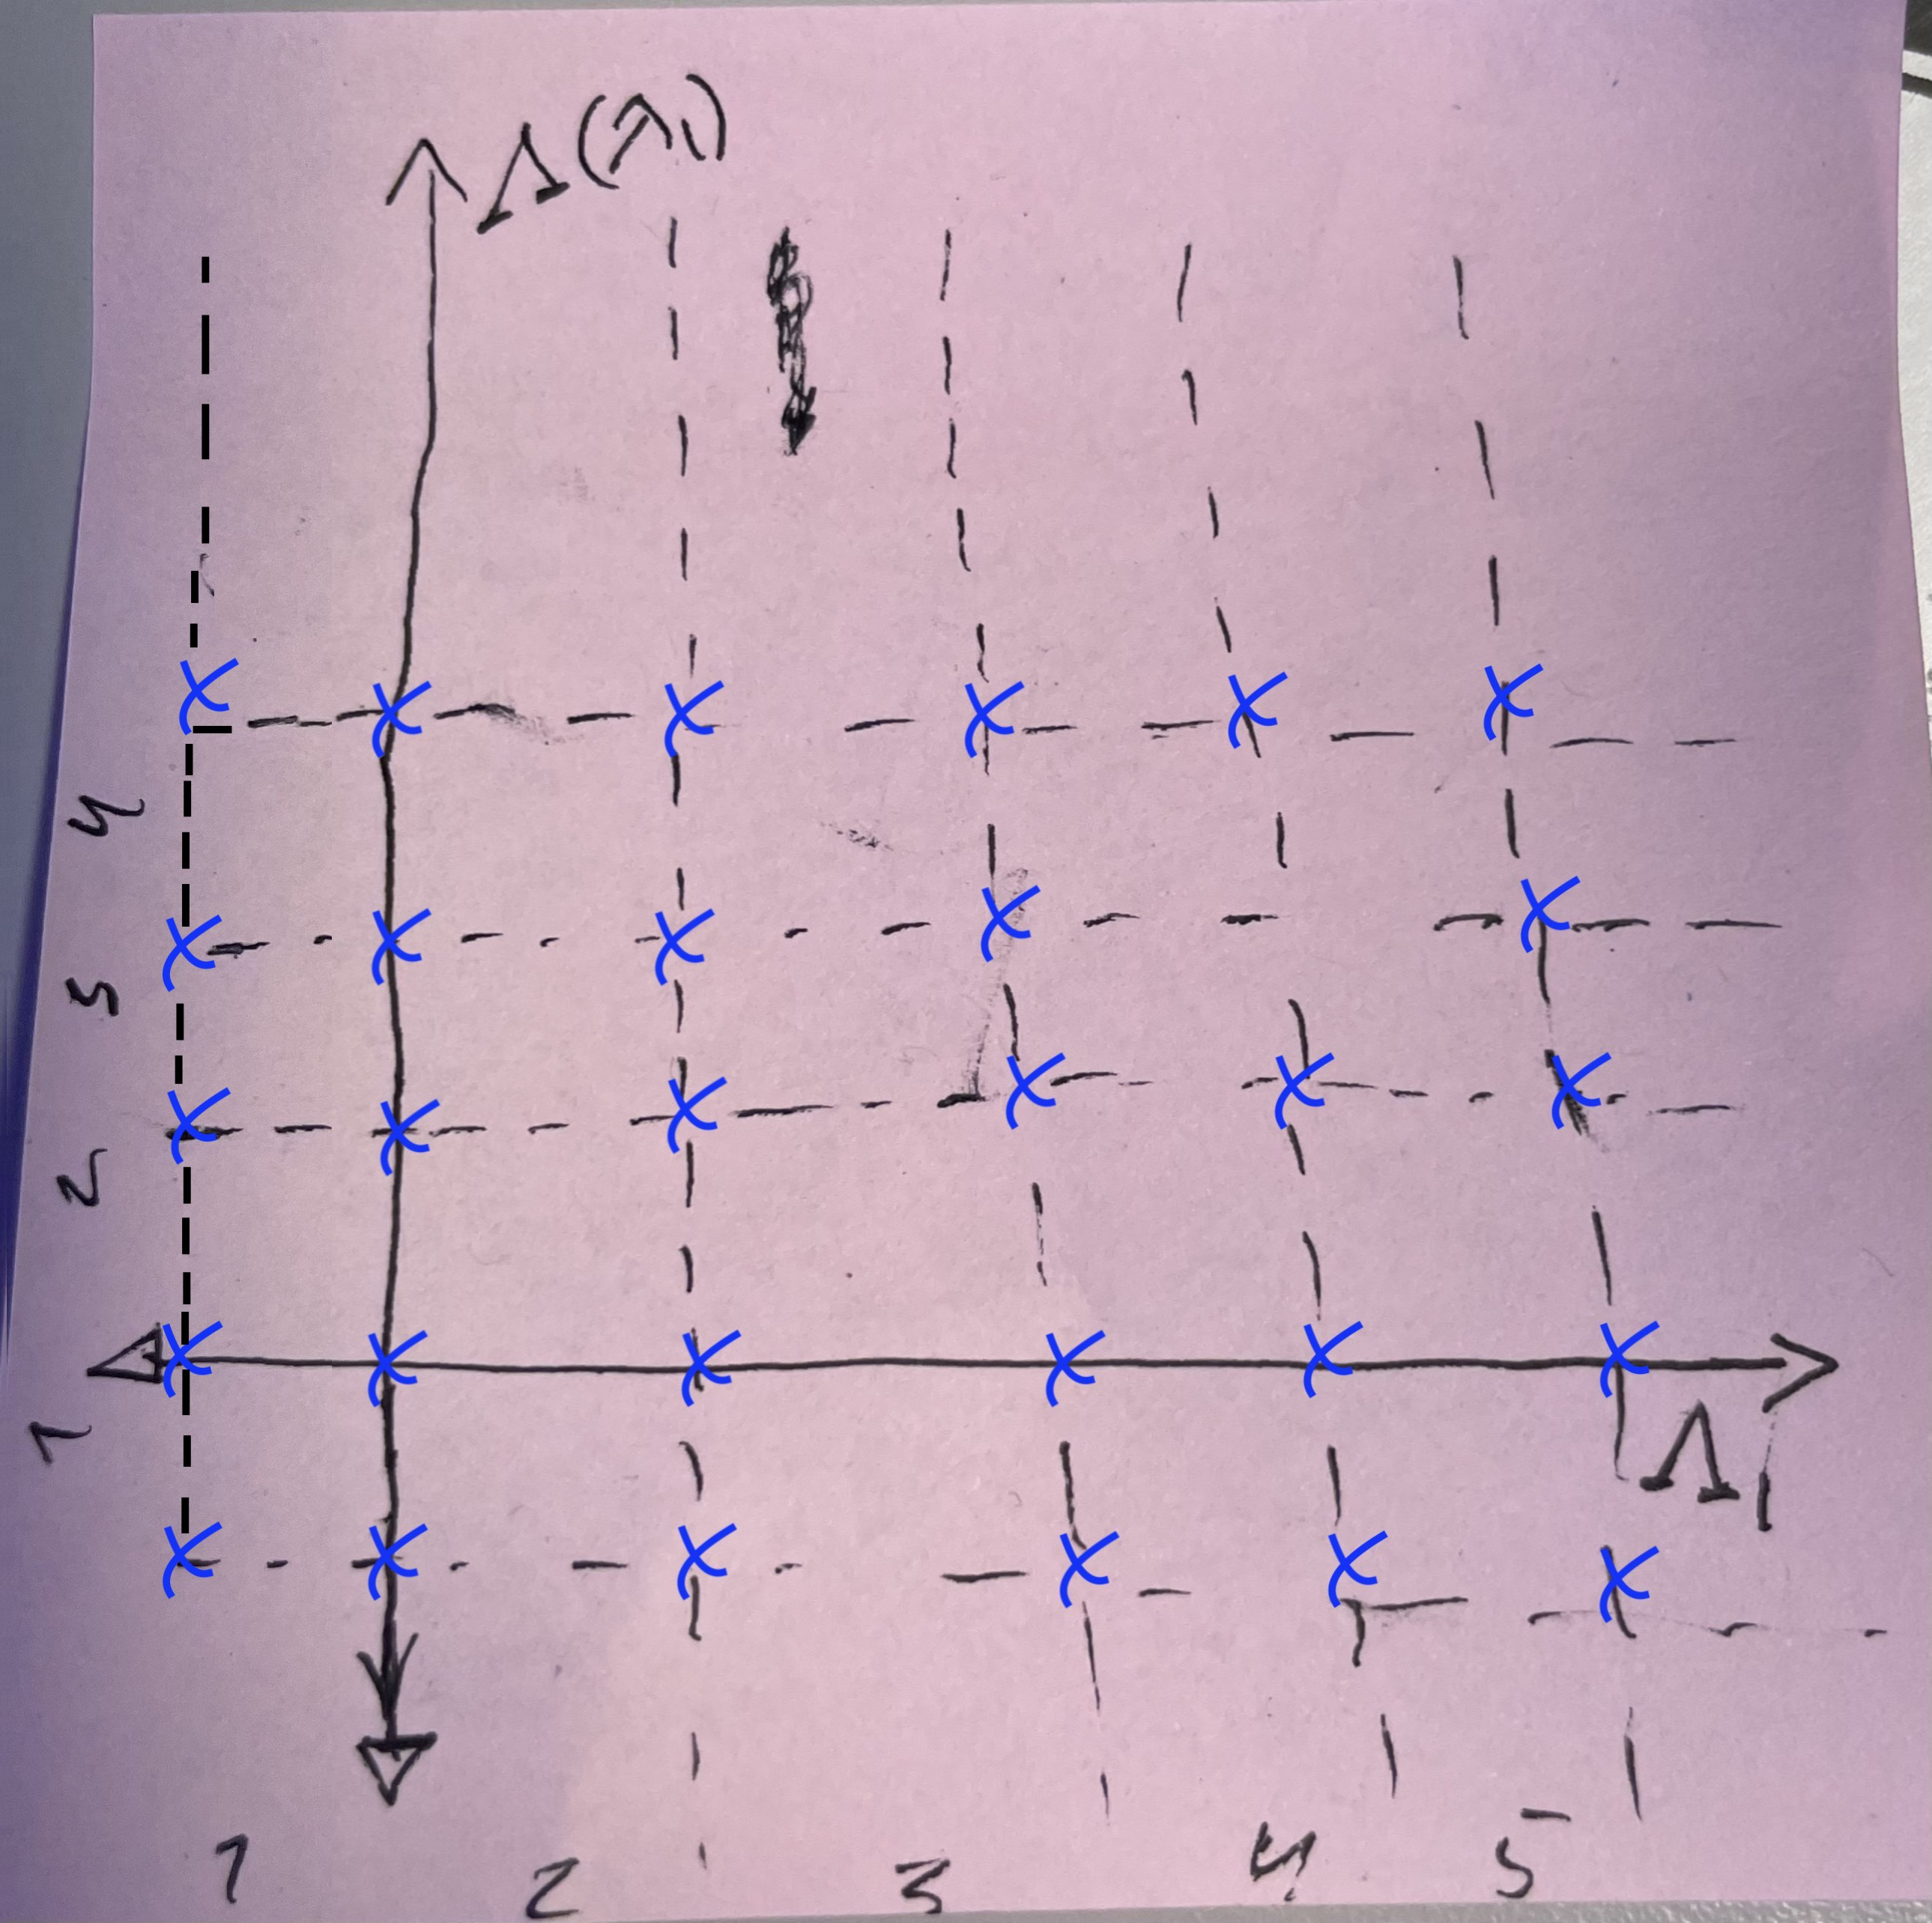
\includegraphics[width=0.9\linewidth]{spec_no_shift.jpg}
        %* Figure 1
        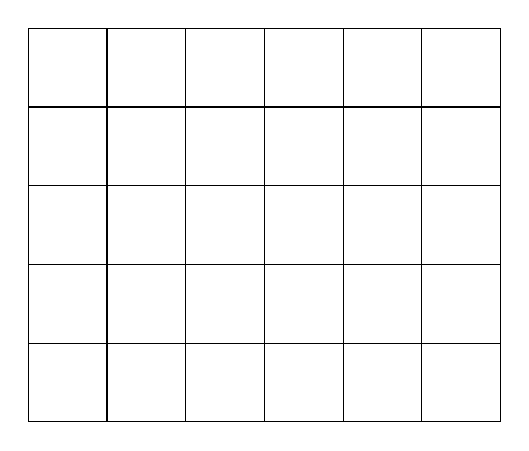
\begin{tikzpicture}[scale=1]
            % Define the tile
            \def\tile{
              % Draw the unit square
              \draw (0,0) rectangle (1,1);
            }
          
            % Draw the tiling pattern
            \foreach \x in {0,1,2,3,4,5}{
              \foreach \y in {0,1,2,3,4}{
                \pgfmathsetmacro{\shiftX}{\x} % Set horizontal shift
                \pgfmathsetmacro{\shiftY}{\y} % Set vertical shift
                \begin{scope}[shift={(\shiftX,\shiftY)}]
                  \tile % Draw the tile
                \end{scope}
              }
            }
        \end{tikzpicture}
        %* —————————————————
        \caption{Lattice tiling}
        \label{fig:tiling_one}
    \end{subfigure}\quad
    \begin{subfigure}{.47\textwidth}
        \centering
        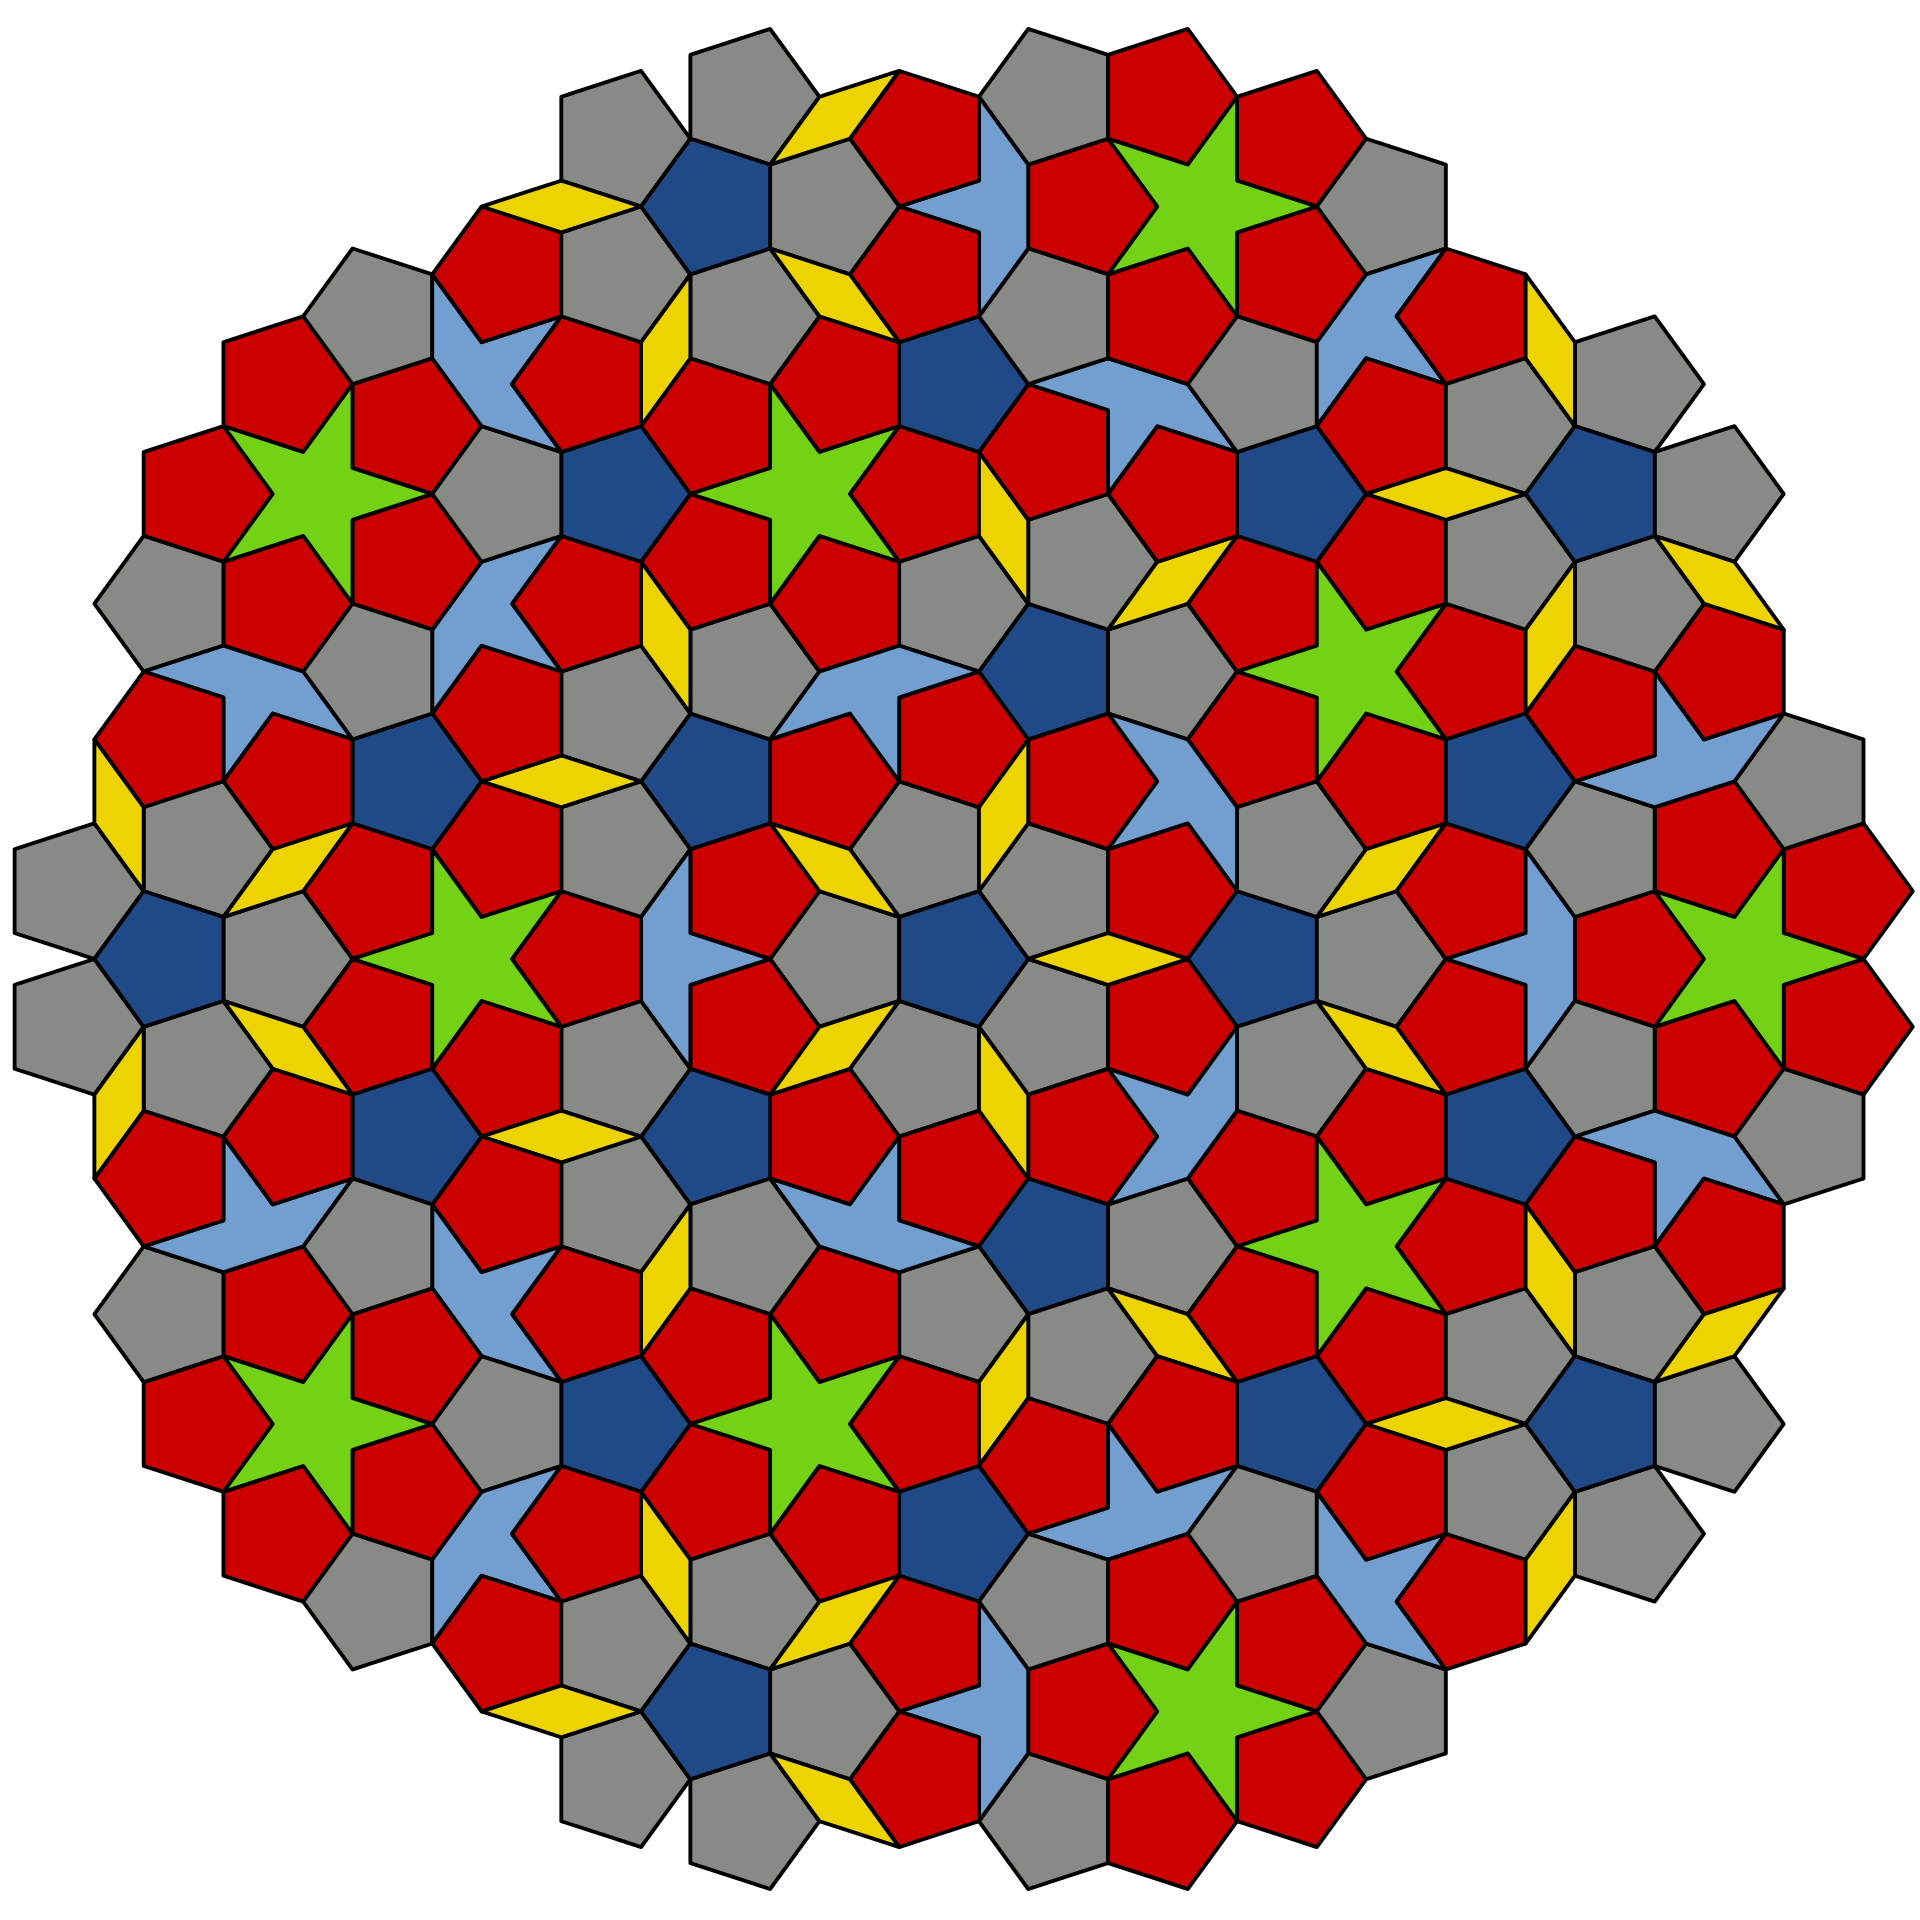
\includegraphics[width=0.87\linewidth]{Penrose_Tiling_.png}
        \caption{P1 Penrose tiling \cite{inductiveloadP1TilingUsing}}
        \label{fig:tiling_two}
    \end{subfigure}
    \caption{Two contrasting tilings of the plane to emphasize the range of complexity. \cref{fig:tiling_one} shows a simple monohedral tiling, and \labelcref{fig:tiling_two} shows an intricate, non-periodic tiling using four different tiles. The coloring in the latter is used to distinguish the tiles more easily and highlight the three \emph{matching rules} for the pentagonal tiles, the only ones with different colors for the same shape. Matching rules are needed in order to tile aperiodically \cite{penrosePentaplexityClassNonPeriodic1979}.}
    \label{fig:tilings_one_two}
\end{figure}

% Penrose goes into the details of these in his paper 

\mycomment{  %! Block comment
The lattice tiling in \labelcref{fig:tiling_one} has fewer tiles and lacks variety compared to Penrose's original aperiodic tiling.

Two tilings of the plane to emphasize the contrast between monohedral tilings and an intricate tiling
Two tilings of the plane emphasize the contrast from monohedral tilings to more intricate tilings, such as the Penrose tiling in Fig. 

Two contrasting tilings of the plane between a monohedral tiling in \cref{fig:tiling_one} and more intricate tilings such as the Penrose tiling in \cref{fig:tiling_two} 

In contrast to the simple monohedral tiling shown in \cref{fig:tiling_one}, the Penrose tiling in \cref{fig:tiling_two} and other intricate tilings provide contrasting examples of tilings on the plane.
In contrast to the simple monohedral tiling shown in \cref{fig:tiling_one}, the Penrose tiling in \cref{fig:tiling_two} is a contrasting example of a more intricate tiling of the plane. 
In contrast to the simple monohedral tiling shown in \cref{fig:tiling_one}, the Penrose tiling in \cref{fig:tiling_two} is an example of a more intricate tiling of the plane. 

Two contrasting tilings of the plane to emphasize the stark difference between a simple monohedral tiling in \cref{fig:tiling_one} and more intricate tilings such as the Penrose tiling in \cref{fig:tiling_two}.
Two contrasting tilings of the plane to emphasize the stark difference between a simple monohedral tiling in \cref{fig:tiling_one} and a more intricate tiling in \cref{fig:tiling_two} which is non-periodic and uses four tiles. 

To emphasize the stark difference between a simple monohedral tiling in \cref{fig:tiling_one} and a more intricate tiling in \cref{fig:tiling_two} which is non-periodic and uses four tiles, we present two contrasting tilings of the plane.

Two contrasting tilings of the plane to emphasize the range of complexity. \cref{fig:tiling_one} shows a simple monohedral tiling, and \cref{fig:tiling_two} shows an intricate, non-periodic tiling using four different tiles. 
} 

Another interesting pair of monohedral tilings is given in \cref{fig:tiling_three,fig:tiling_four}. These are both examples of an Escher tiling in which a lizard and horseman tile the plane. Note that in comparison to the square tilings in \cref{fig:tiling_one}, there is important to highlight two fundamental differences between the square and Escher tilings. The first is that one needs to rotate the lizard to cover the entire surface, and the second is that one needs to reflect the horseman to cover the entire surface. It is these three motions and combinations of them that we use when tiling in general \cite[p. 26]{kolountzakisTilingsTranslation2010,grunbaumTilingsPatterns1987}. 




\begin{figure}[t]%h!
    \centering
    \begin{subfigure}{.47\textwidth}
        \centering
        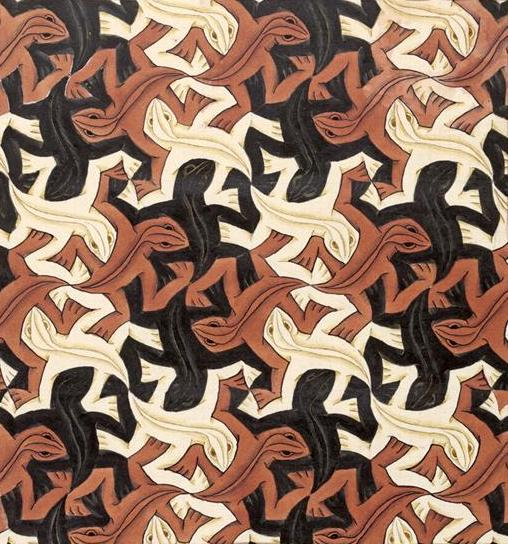
\includegraphics[width=0.9\linewidth]{lizard-1.jpg}
        \caption{Lizard}
        \label{fig:tiling_three}
    \end{subfigure}\quad
    \begin{subfigure}{.47\textwidth}
        \centering
        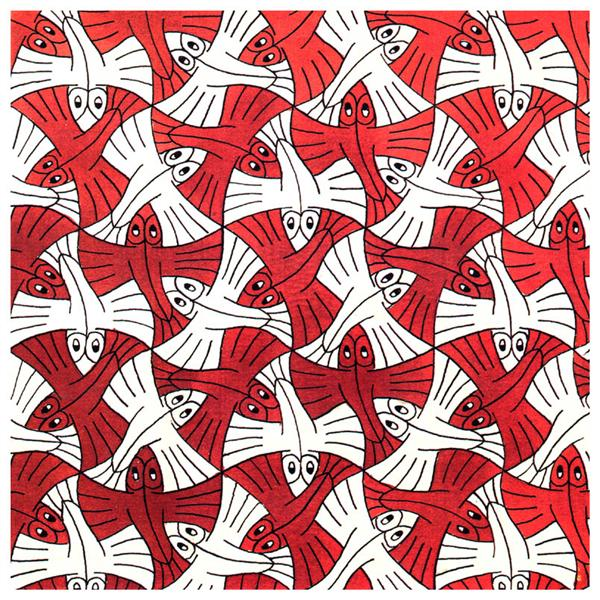
\includegraphics[width=0.9\linewidth]{flying-fish.jpg}
        \caption{Flying fish}
        \label{fig:tiling_four}
    \end{subfigure}
    \caption{Text}
    \label{fig:tilingsss_two}
\end{figure}

However interesting the Penrose and Escher tilings appear, we will only focus on monohedral tilings of $\R^d$ by translation, using the unit cube as our tile. Considering only cube-tilings might seem simple initially, but we will see that as we increase the dimension, we get increased flexibility and more complex tilings. It turns out that in higher dimensions, highly exotic and counterintuitive cube tilings exist. The fact that this kind of tiling exists in the first place is surprising in light of Keller's \namecref{thrm:keller_tiling} \cite{iosevichSpectralTilingProperties1998}.  % This is Perhaps surprising in light of Keller's \namecref{thrm:keller_tiling}. 

%\begin{theorem}  %* (My original) Keller theorem from the paper of Iosovich and Pedersen
%    Given a discrete subset $T\subset \R^d$. If $T$ is a tiling set for $\Omega$, then given any pair $\lambda, \lambda' \in T$ such that $\lambda\neq\lambda'$, there exists a $j\in \braq{1,\dots,d}$ so that $\bral{t_j -t_j' } \in \N$
%\end{theorem}
%\begin{theorem}  %* Keller theorem from the paper of Lagarias and Reeds
%    If $\Lambda + \bras{0,1}^n$ is a tiling of $\R^n$, then each $\lambda,\lambda'\in \Lambda$ has
%    \begin{equation*}
%        \lambda_i - \lambda_i' \in \intnozero \quad \text{ for some } i, \quad 1\leq i \leq n.
%    \end{equation*}
%\end{theorem}
\begin{theorem}[Keller's theorem]\label{thrm:keller_tiling}
    %Let $\Lambda \subset \R^d$ be a discrete subset.  %* No need to specify, as we will define the tiling set later
    If $\Lambda$ is a tiling set for the unit cube, then for any two $\lambda, \lambda' \in \Lambda$ with $\lambda\neq\lambda'$, there exist a $j\in \braq{1,\dots,d}$ so that $\lambda_j-\lambda_j' \in \intnozero$.
\end{theorem}

We will formally define what we mean by a \emph{tiling set} from \cref{thrm:keller_tiling} later (\cref{def:tiling}), but for now, we continue this informal discussion on exotic tilings. Now, although Keller proved the theorem in his original paper \cite{kellerUberLuckenloseErfullung1930}, Iosevich and Pedersen provide an English proof in their paper \cite{iosevichSpectralTilingProperties1998}. Furthermore, in the same paper by Keller, he also conjectured the following. 

\begin{conjecture}[Keller's conjecture]\label{conj:keller_tiling}
    All tilings of $\R^d$ by translations of the unit cube contain \textsc{two} cubes that share an entire $(d-1)$-dimensional face.
\end{conjecture}  %* For å kaste lys på at de kan være eksotiske så er det det at de er usant over 7 som er det relevante her. 


% fill=gray!50

\begin{figure}[t!]%h!
    \centering
    \begin{subfigure}{.47\textwidth}
        \centering
        %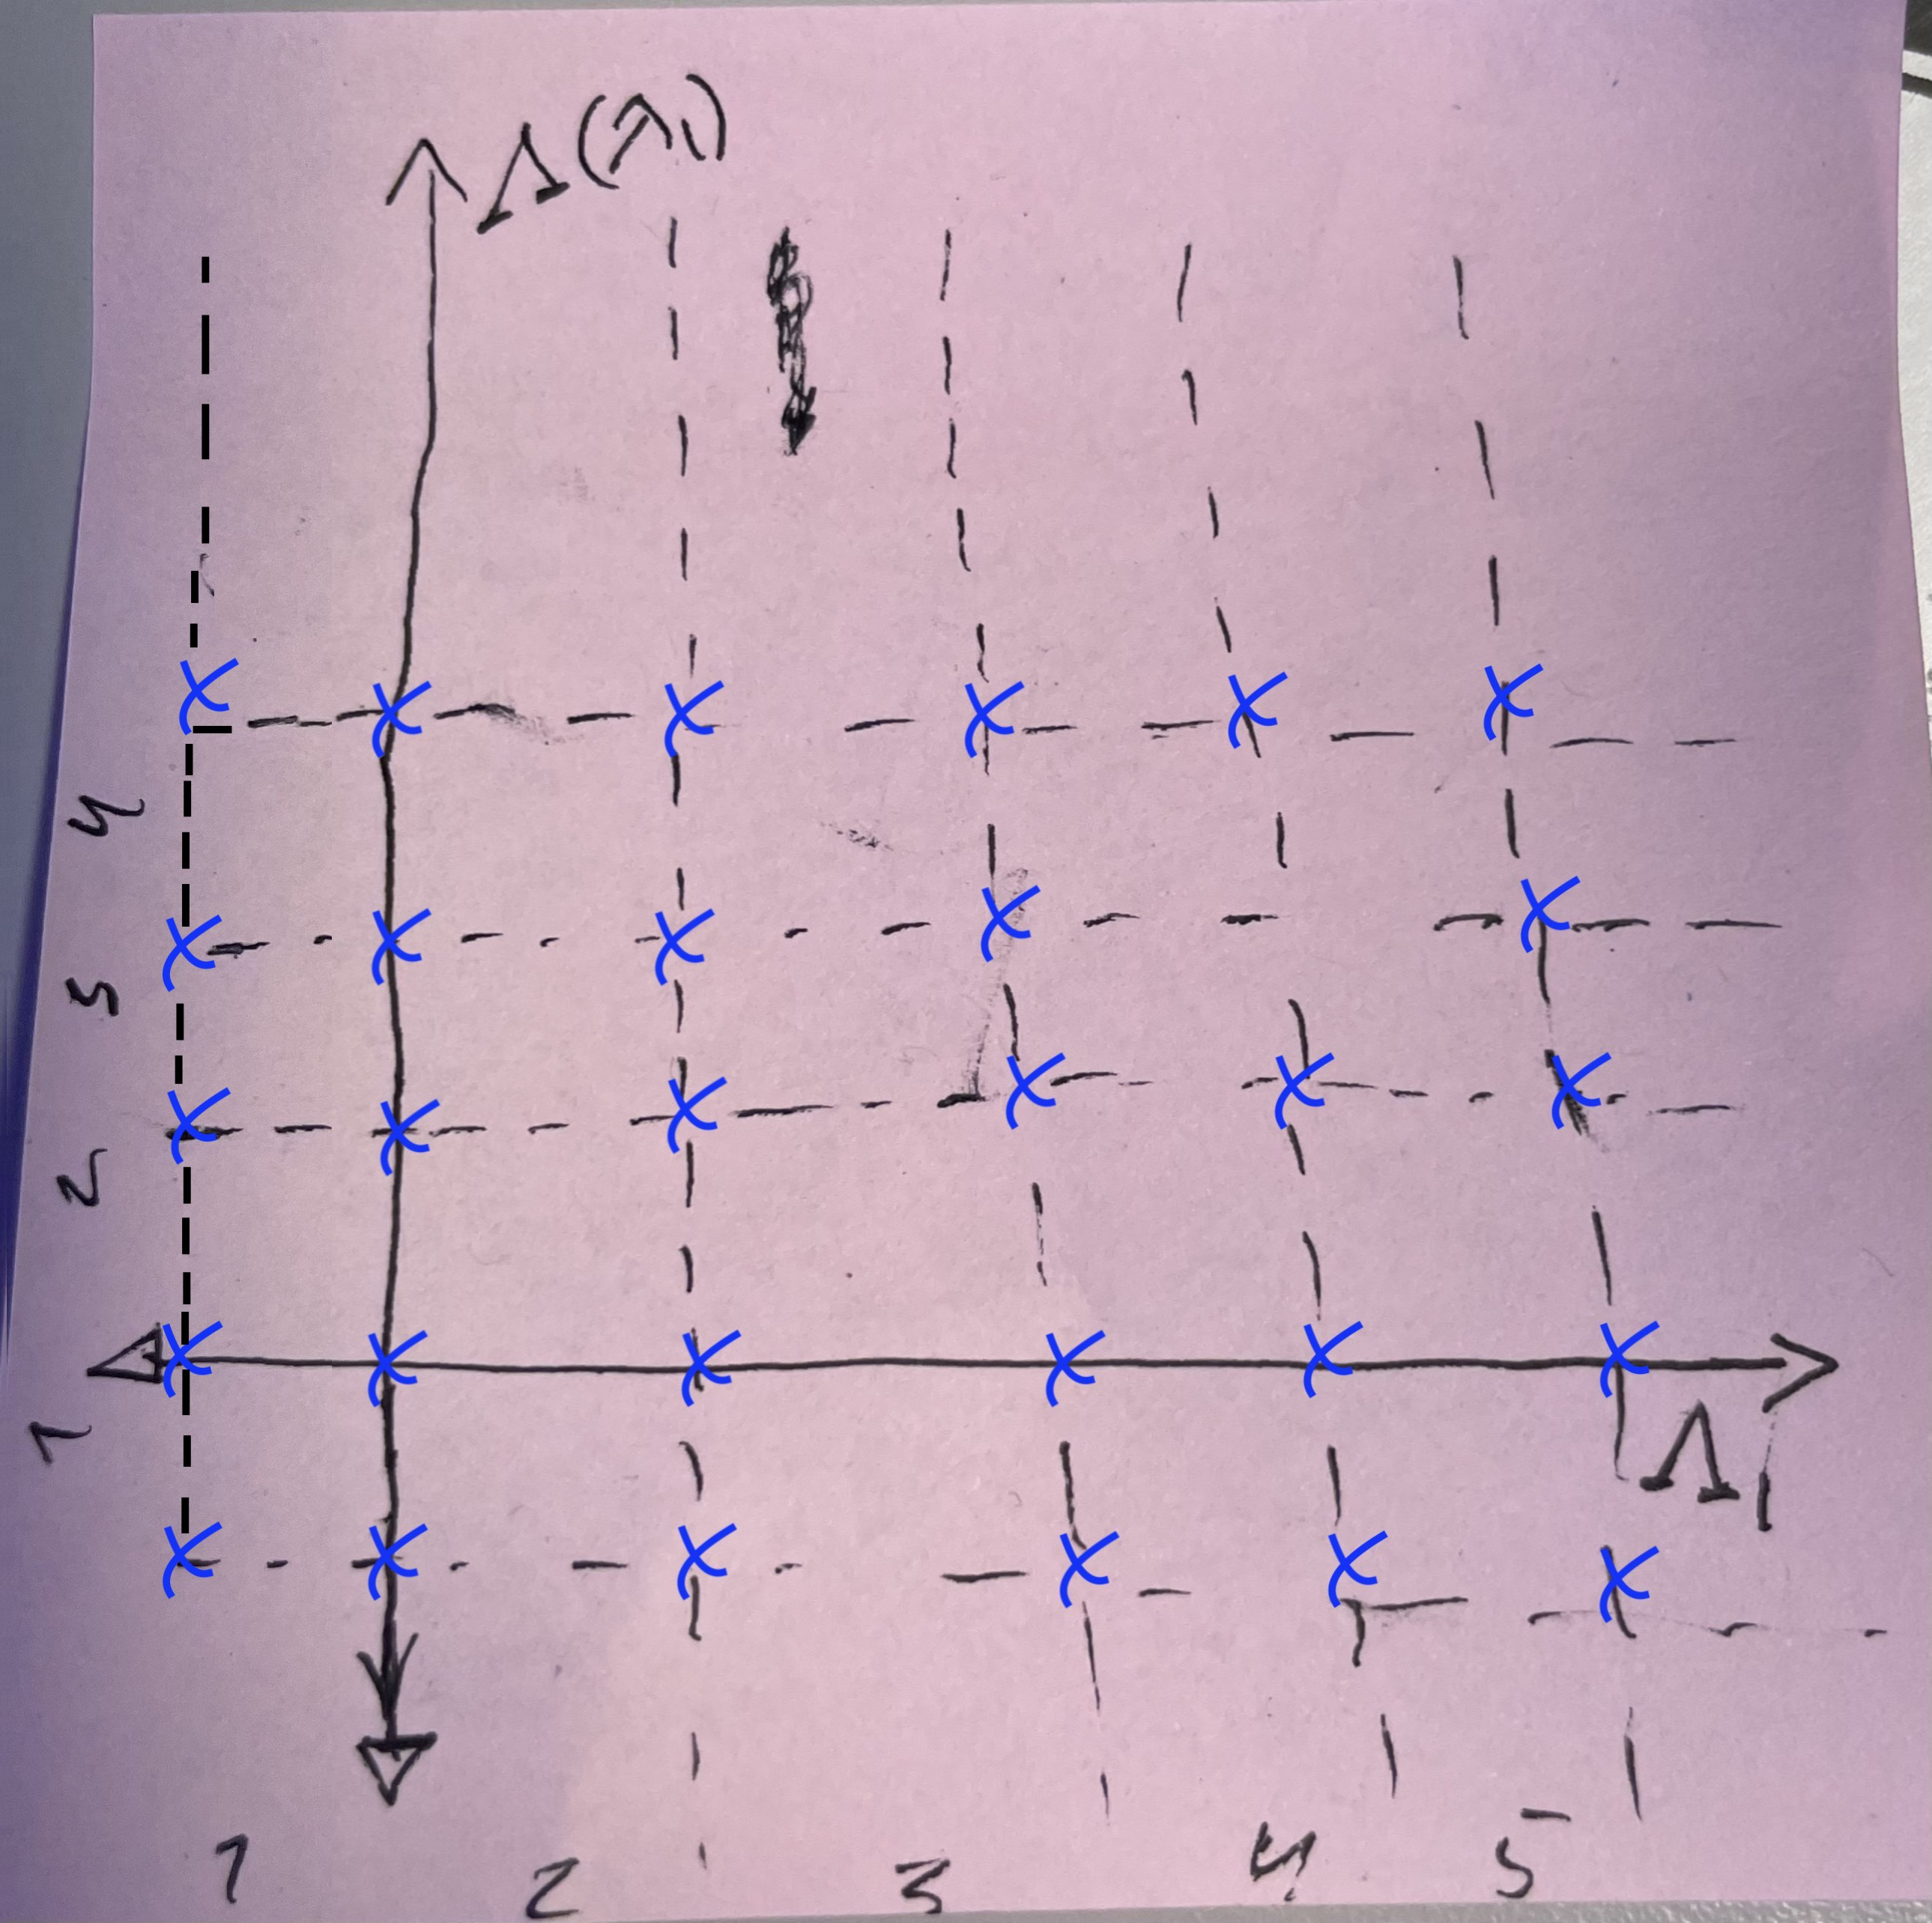
\includegraphics[width=0.9\linewidth]{spec_no_shift.jpg}
        %* Figure 1
        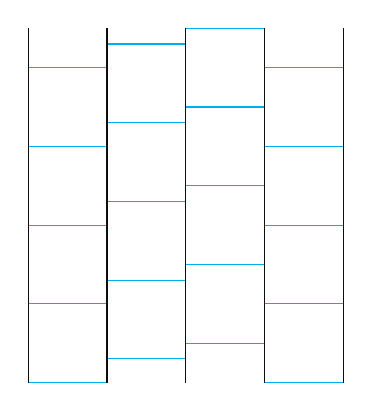
\begin{tikzpicture}[scale=1]
            % Define the tile
            \def\tile{
            %\draw (1,0) -- (1,1) -- (0,1) -- (0,0) -- cycle;  % Draw the unit square
            \draw[black!95] (0,0) rectangle (1,1);
            %\draw (0,0) rectangle (1,1);
            \draw[cyan] (0,0) -- (1,0);
            \draw[cyan] (0,1) -- (1,1);
            }
            
            % Draw the tiling pattern
            \foreach \x in {0,1,2,3}{
                \foreach \y in {0,1,2,3}{
                    % Here we shift with different z values for each height value 
                    % i.e. Row shift
                    \ifnum\x=0
                        \pgfmathsetmacro{\shiftX}{\x} % Set horizontal shift
                        \pgfmathsetmacro{\shiftY}{\y}
                    \fi
                    \ifnum\x=1
                        \pgfmathsetmacro{\shiftX}{\x} % Set horizontal shift
                        \pgfmathsetmacro{\shiftY}{\y+0.3}
                    \fi
                    \ifnum\x=2
                        \pgfmathsetmacro{\shiftX}{\x} % Set horizontal shift
                        \pgfmathsetmacro{\shiftY}{\y+0.5}
                    \fi
                    \ifnum\x=3
                        \pgfmathsetmacro{\shiftX}{\x} % Set horizontal shift
                        \pgfmathsetmacro{\shiftY}{\y}
                    \fi
                    \begin{scope}[shift={(\shiftX,\shiftY)}]
                        \tile % Draw the tile
                    \end{scope}
                }
            }
            % black lines to hide the blue lines
            \foreach \x in {0,1,2,3,4}{
                \draw[ black!95] (\x,0) -- (\x,4);
                \draw[black!95] (\x,0+0.3) -- (\x,4+0.3);
                \draw[black!95] (\x,0+0.3) -- (\x,4+0.5);
                \draw[black!95] (\x,0) -- (\x,4+0.5);
                \draw[black!95] (\x,0) -- (\x,4);
            }
        \end{tikzpicture}
        %* —————————————————
        %\caption{Lattice tiling}
        \label{fig:tiling_five}
    \end{subfigure}\quad
    \begin{subfigure}{.47\textwidth}
        \centering
        %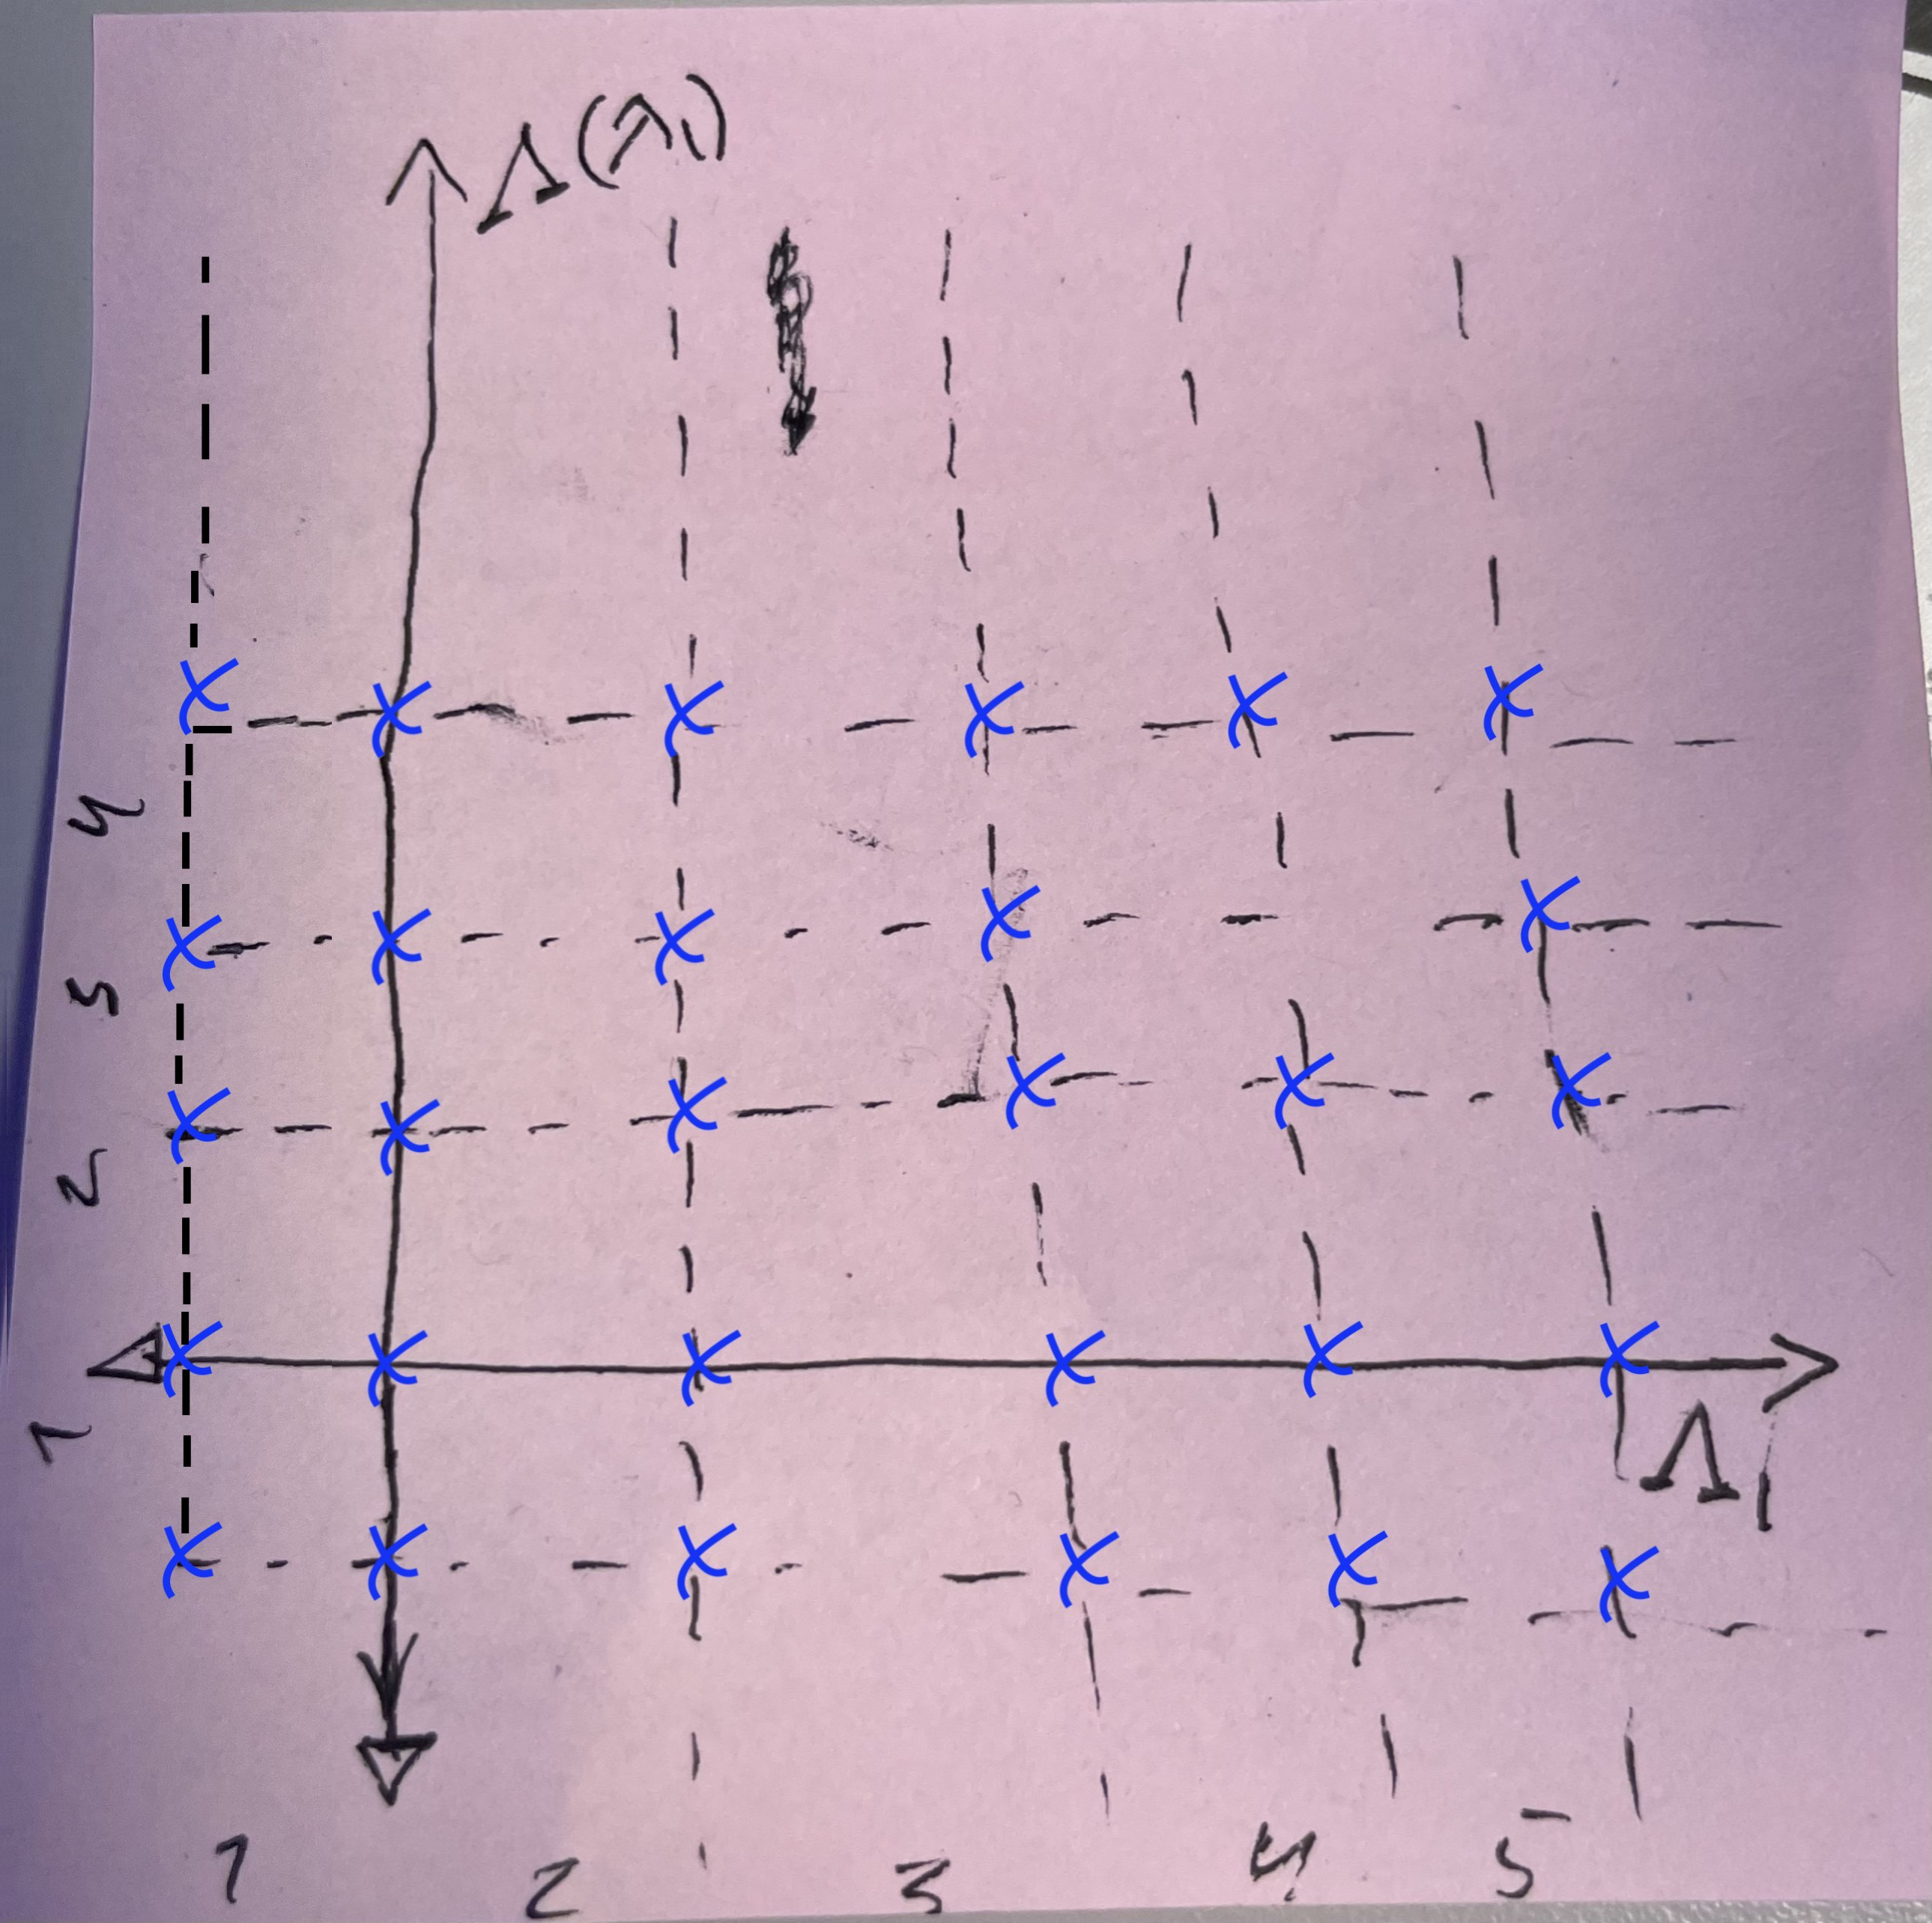
\includegraphics[width=0.9\linewidth]{spec_no_shift.jpg}
        %* Figure 1
        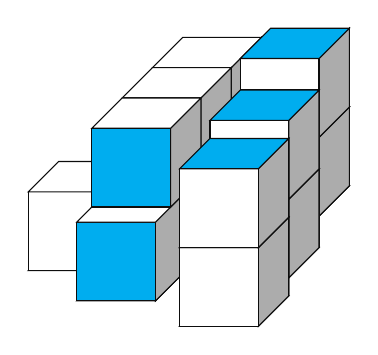
\begin{tikzpicture}[scale=1]
            % Define the tile
            \def\tile{
              % Draw the unit cube
                \draw[black!95] (1,0,0) -- (1,0,1) -- (1,1,1) -- (1,1,0) -- cycle; % left face
                \draw[black!95] (0,0,0) -- (1,0,0) -- (1,0,1) -- (0,0,1) -- cycle; % bottom face
                \draw[black!95] (0,0,0) -- (0,1,0) -- (1,1,0) -- (1,0,0) -- cycle; % back face
                \draw[black!95, fill=gray!65] (1,0,0) -- (1,1,0) -- (1,1,1) -- (1,0,1) -- cycle; % right face
                \draw[black!95, fill=white] (0,0,1) -- (1,0,1) -- (1,1,1) -- (0,1,1) -- cycle; % front face
                \draw[black!95, fill=white](0,1,0) -- (0,1,1) -- (1,1,1) -- (1,1,0) -- cycle; % top face
            }
            
            \def\tiletwo{
                % Draw the unit cube
                    \draw[black!95] (1,0,0) -- (1,0,1) -- (1,1,1) -- (1,1,0) -- cycle; % left face
                    \draw[black!95] (0,0,0) -- (1,0,0) -- (1,0,1) -- (0,0,1) -- cycle; % bottom face
                    \draw[black!95] (0,0,0) -- (0,1,0) -- (1,1,0) -- (1,0,0) -- cycle; % back face
                    \draw[black!95, fill=gray!65] (1,0,0) -- (1,1,0) -- (1,1,1) -- (1,0,1) -- cycle; % right face
                    \draw[black!95, fill=cyan] (0,0,1) -- (1,0,1) -- (1,1,1) -- (0,1,1) -- cycle; % front face
                    \draw[black!95, fill=white](0,1,0) -- (0,1,1) -- (1,1,1) -- (1,1,0) -- cycle; % top face
                }
        
            \def\tilethree{
                % Draw the unit cube
                    \draw[black!95] (1,0,0) -- (1,0,1) -- (1,1,1) -- (1,1,0) -- cycle; % left face
                    \draw[black!95] (0,0,0) -- (1,0,0) -- (1,0,1) -- (0,0,1) -- cycle; % bottom face
                    \draw[black!95] (0,0,0) -- (0,1,0) -- (1,1,0) -- (1,0,0) -- cycle; % back face
                    \draw[black!95, fill=gray!65] (1,0,0) -- (1,1,0) -- (1,1,1) -- (1,0,1) -- cycle; % right face
                    \draw[black!95, fill=white] (0,0,1) -- (1,0,1) -- (1,1,1) -- (0,1,1) -- cycle; % front face
                    \draw[black!95, fill=cyan](0,1,0) -- (0,1,1) -- (1,1,1) -- (1,1,0) -- cycle; % top face
                }
          
            % Draw the tiling pattern
            % For x=0
            \foreach \x in {0}{
               \foreach \y in {0}{
                    \foreach \z in {0}{
                        \pgfmathsetmacro{\shiftX}{\x} % Set horizontal shift
                        \pgfmathsetmacro{\shiftY}{\y} % Set vertical shift
                        \pgfmathsetmacro{\shiftZ}{\z+0.8} % Set vertical shift
                        \begin{scope}[shift={(\shiftX,\shiftY,\shiftZ)}]
                        \tile % Draw the tile
                        \end{scope}
                    }
                }
            }
            % For x=1
            \foreach \x in {1}{
               \foreach \y in {0,1}{
                    \foreach \z in {-1,0,1}{
                        % Here we shift with different z values for each height value 
                        % i.e. Row shift
                        \ifnum\y=0
                            \pgfmathsetmacro{\shiftX}{\x} % Set horizontal shift
                            \pgfmathsetmacro{\shiftY}{\y}
                            \pgfmathsetmacro{\shiftZ}{\z+0.8} % Set vertical shift
                        \fi
                        \ifnum\y=1
                            \pgfmathsetmacro{\shiftX}{\x} % Set horizontal shift
                            \pgfmathsetmacro{\shiftY}{\y}
                            \pgfmathsetmacro{\shiftZ}{\z+0.3} % Set vertical shift
                        \fi
                        \ifnum\y=2
                            \pgfmathsetmacro{\shiftX}{\x} % Set horizontal shift
                            \pgfmathsetmacro{\shiftY}{\y}
                            \pgfmathsetmacro{\shiftZ}{\z-0.5} % Set vertical shift
                        \fi
                        
                        \begin{scope}[shift={(\shiftX,\shiftY,\shiftZ)}]
                        \tiletwo % Draw the tile
                        \end{scope}
                    }
                }
            }
        
            % For x=2
            % The code for this part is a bit divided, thre last columns are here, the one in the very back has same shift as the one in the front
            \foreach \x in {2}{
               \foreach \y in {0,1}{
                    \foreach \z in {-1,0,1}{
                        % Here we shift with different y values for each depth value
                        % i.e. Column shift
                        \ifnum\z=-1
                            \pgfmathsetmacro{\shiftX}{\x} % Set horizontal shift
                            \pgfmathsetmacro{\shiftY}{\y}
                            \pgfmathsetmacro{\shiftZ}{\z} % Set vertical shift
                        \fi
                        \ifnum\z=0
                            \pgfmathsetmacro{\shiftX}{\x} % Set horizontal shift
                            \pgfmathsetmacro{\shiftY}{\y-0.4}
                            \pgfmathsetmacro{\shiftZ}{\z} % Set vertical shift
                        \fi
                        \ifnum\z=1
                            \pgfmathsetmacro{\shiftX}{\x} % Set horizontal shift
                            \pgfmathsetmacro{\shiftY}{\y-0.63}
                            \pgfmathsetmacro{\shiftZ}{\z} % Set vertical shift
                        \fi
                        \begin{scope}[shift={(\shiftX,\shiftY,\shiftZ)}]
                        \tilethree % Draw the tile
                        \end{scope}
                    }
                }
            }
        \end{tikzpicture}
        %* —————————————————
        %\caption{Lattice tiling}
        \label{fig:tiling_six}
    \end{subfigure}
    \caption{Highlighted in cyan are the fully face-sharing edges (left) and squares (right) for $d=2$ and $d=3$, respectively. Observe the two different orientations for the cyan squares.}
    \label{fig:tilings_five_six}
\end{figure}


If the dimension is two, the squares share an edge; if the dimension is three, they share a square. \cref{fig:tilings_five_six} illustrates this. Furthermore, when $d\geq 3$, it is not necessarily true that \emph{all} cubes shared a whole $(n-1)$-dimensional face with one of its neighbors \cite{perronUeberLueckenloseAusfuellung1940}. It is important to emphasize that the conjecture does not support the existence of exotic tilings. Instead, it indicates the opposite — rigidity in the tiling of the space. %/ $\R^d$.
However, after being first proven true for $d\leq 6$ by Perron in 1940 \cite{perronModulartigeLueckenloseAusfuellung1940,perronModulartigeLueckenloseAusfuellung1940a}, it has since then gradually been proved false for all $d\geq10$ \cite{lagariasKellerCubetilingConjecture1992} and later all $d\geq8$ \cite{mackeyCubeTilingDimension2002}. The last remaining dimension was finally solved in 2020, where it was proven to be true \cite{brakensiekResolutionKellerConjecture2020}, leading us to a solution in all dimensions for Keller's \namecref{conj:keller_tiling}.%, \cref{conj:keller_tiling}. 

\begin{theorem}
    In all tilings of $\R^d$ by translations of the unit cube, Keller's \namecref{conj:keller_tiling}, \cref{conj:keller_tiling}, is true for all dimensions $d\leq 7$ and false for all $d>7$.
\end{theorem}

%* Longer explanation: "An example of what..."
%While we refer to \cite{brakensiekResolutionKellerConjecture2020} for a comprehensive and detailed exposition on how Keller's conjecture has been reduced and transformed into a graph theoretic problem solved using computer-aided mathematics, to briefly explain the concept and give an example of what these higher-dimensional tilings might look like consider the following: Keller graphs denoted as $G_{d,s}$ consist of vertices given by $\braq{0,1,2,\dots,2s-1}^d$. Here, $d$ is the dimension, and $s$ indicates all the different values a coordinate can take. In this graph, two vertices are considered adjacent if they differ in at least two coordinates, where at least one of these differences must be exactly $s$. Within each graph $G_{d,s}$, we can have cliques of different sizes, but they cannot be larger than $2^d$. However, a clique of size $2^d$ within $G_{d,s}$ would disprove Keller's conjecture for dimensions greater than or equal to that dimension $d$. For dimension $d=8$, a clique of size $2^8=256$ within $G_{8,2}$ is what is depicted in \cref{fig:tiling_seven}. Notably, since $s=2$, this represents the smallest counterexample to Keller's \namecref{conj:keller_tiling}, \cref{conj:keller_tiling}.
\begin{remark}
    Keller also wrote a paper claiming to solve his conjecture for $d\leq 6$ \cite{Keller1937}. However, Perron later described Keller's solution for $d=5$ and $d=6$ as \emph{"quite incomprehensible to me"} and \emph{"very sketchy"} in the literal sense of the word \cite{perronUeberLueckenloseAusfuellung1940} \footnote[1]{Perron's origninal description of Keller's solution to his conjecture: \emph{— Enthält einen sehr skizzenhaften mir ziemlich unverständlichen Beweis für die Richtigkeit der Kellerchen Vermutung im Falle n=5 unt n=6.}}. Furthermore, what is interesting is the fact that Keller himself later doubted whether his conjecture was actually true.
\end{remark}

While we refer to \cite{brakensiekResolutionKellerConjecture2020} for a comprehensive and detailed exposition on how Keller's conjecture has been reduced and transformed into a graph theoretic problem solved using computer-aided mathematics, to briefly explain the concept consider the following: \emph{Keller graphs} denoted as $G_{d,s}$ consist of \emph{vertices} given by $\braq{0,1,2,\dots,2s-1}^d$. Here, $d$ denotes the dimension, and $s$ denotes the number of \emph{coordinates}. In this graph, two vertices are considered \emph{adjacent} if they differ in at least two coordinates, where at least one of these differences must be exactly $s$. Within each graph $G_{d,s}$, we can have \emph{cliques} of different sizes, but they cannot be larger than $2^d$. A clique is a subgraph with any two adjacent vertices. However, a clique of size $2^d$ within $G_{d,s}$ would disprove Keller's conjecture for dimensions greater than or equal to that dimension $d$. This condition is the critical key in resolving the conjecture through Keller graphs \cite{corradiCombinatorialApproachKeller1990}. This combinatorial argument was made possible after Hajos reformulated Keller's \namecref{conj:keller_tiling} into an algebraic equivalent, similar to what he did before solving Minkowski's \namecref{conj:keller_tiling} \cite{lagariasKellerCubetilingConjecture1992,hajosUeberEinfacheUnd1942}. For dimension $d=8$, a clique of size $2^8=256$ within $G_{8,2}$ is what is depicted in \cref{fig:tiling_seven}. Notably, since $s=2$, this also represents the smallest counterexample. %Notably, since $s=2$, this represents the smallest counterexample to Keller's \namecref{conj:keller_tiling}, \cref{conj:keller_tiling}.  %* The coordinate set indicates all the different values a coordinate can take.


% fill=gray!50

\begin{figure}[t!]%h!
    \centering
    \begin{subfigure}{.47\textwidth}
        \centering
        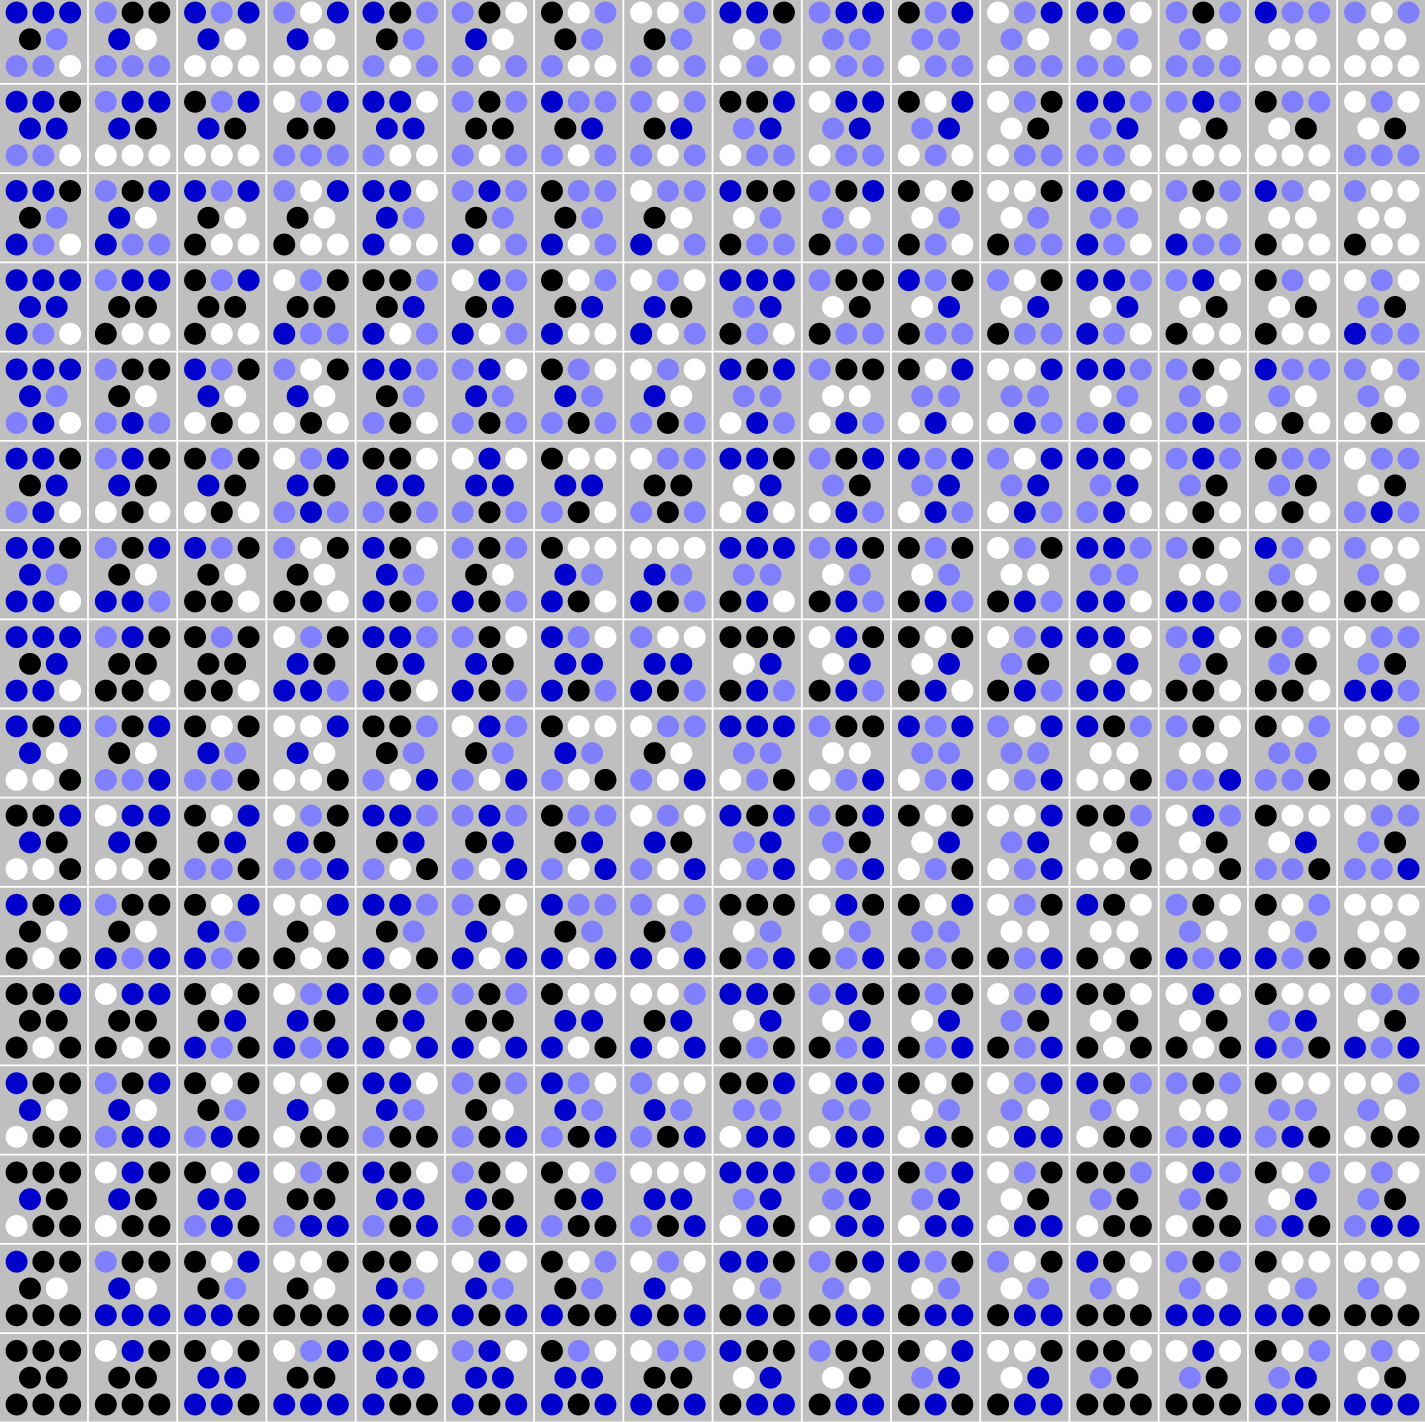
\includegraphics[width=0.9\linewidth]{keller_clique.png}
        %* —————————————————
        \caption{A Keller graph \cite{brakensiekResolutionKellerConjecture2020}}
        \label{fig:tiling_seven}
    \end{subfigure}\quad
    \begin{subfigure}{.47\textwidth}
        \centering
        %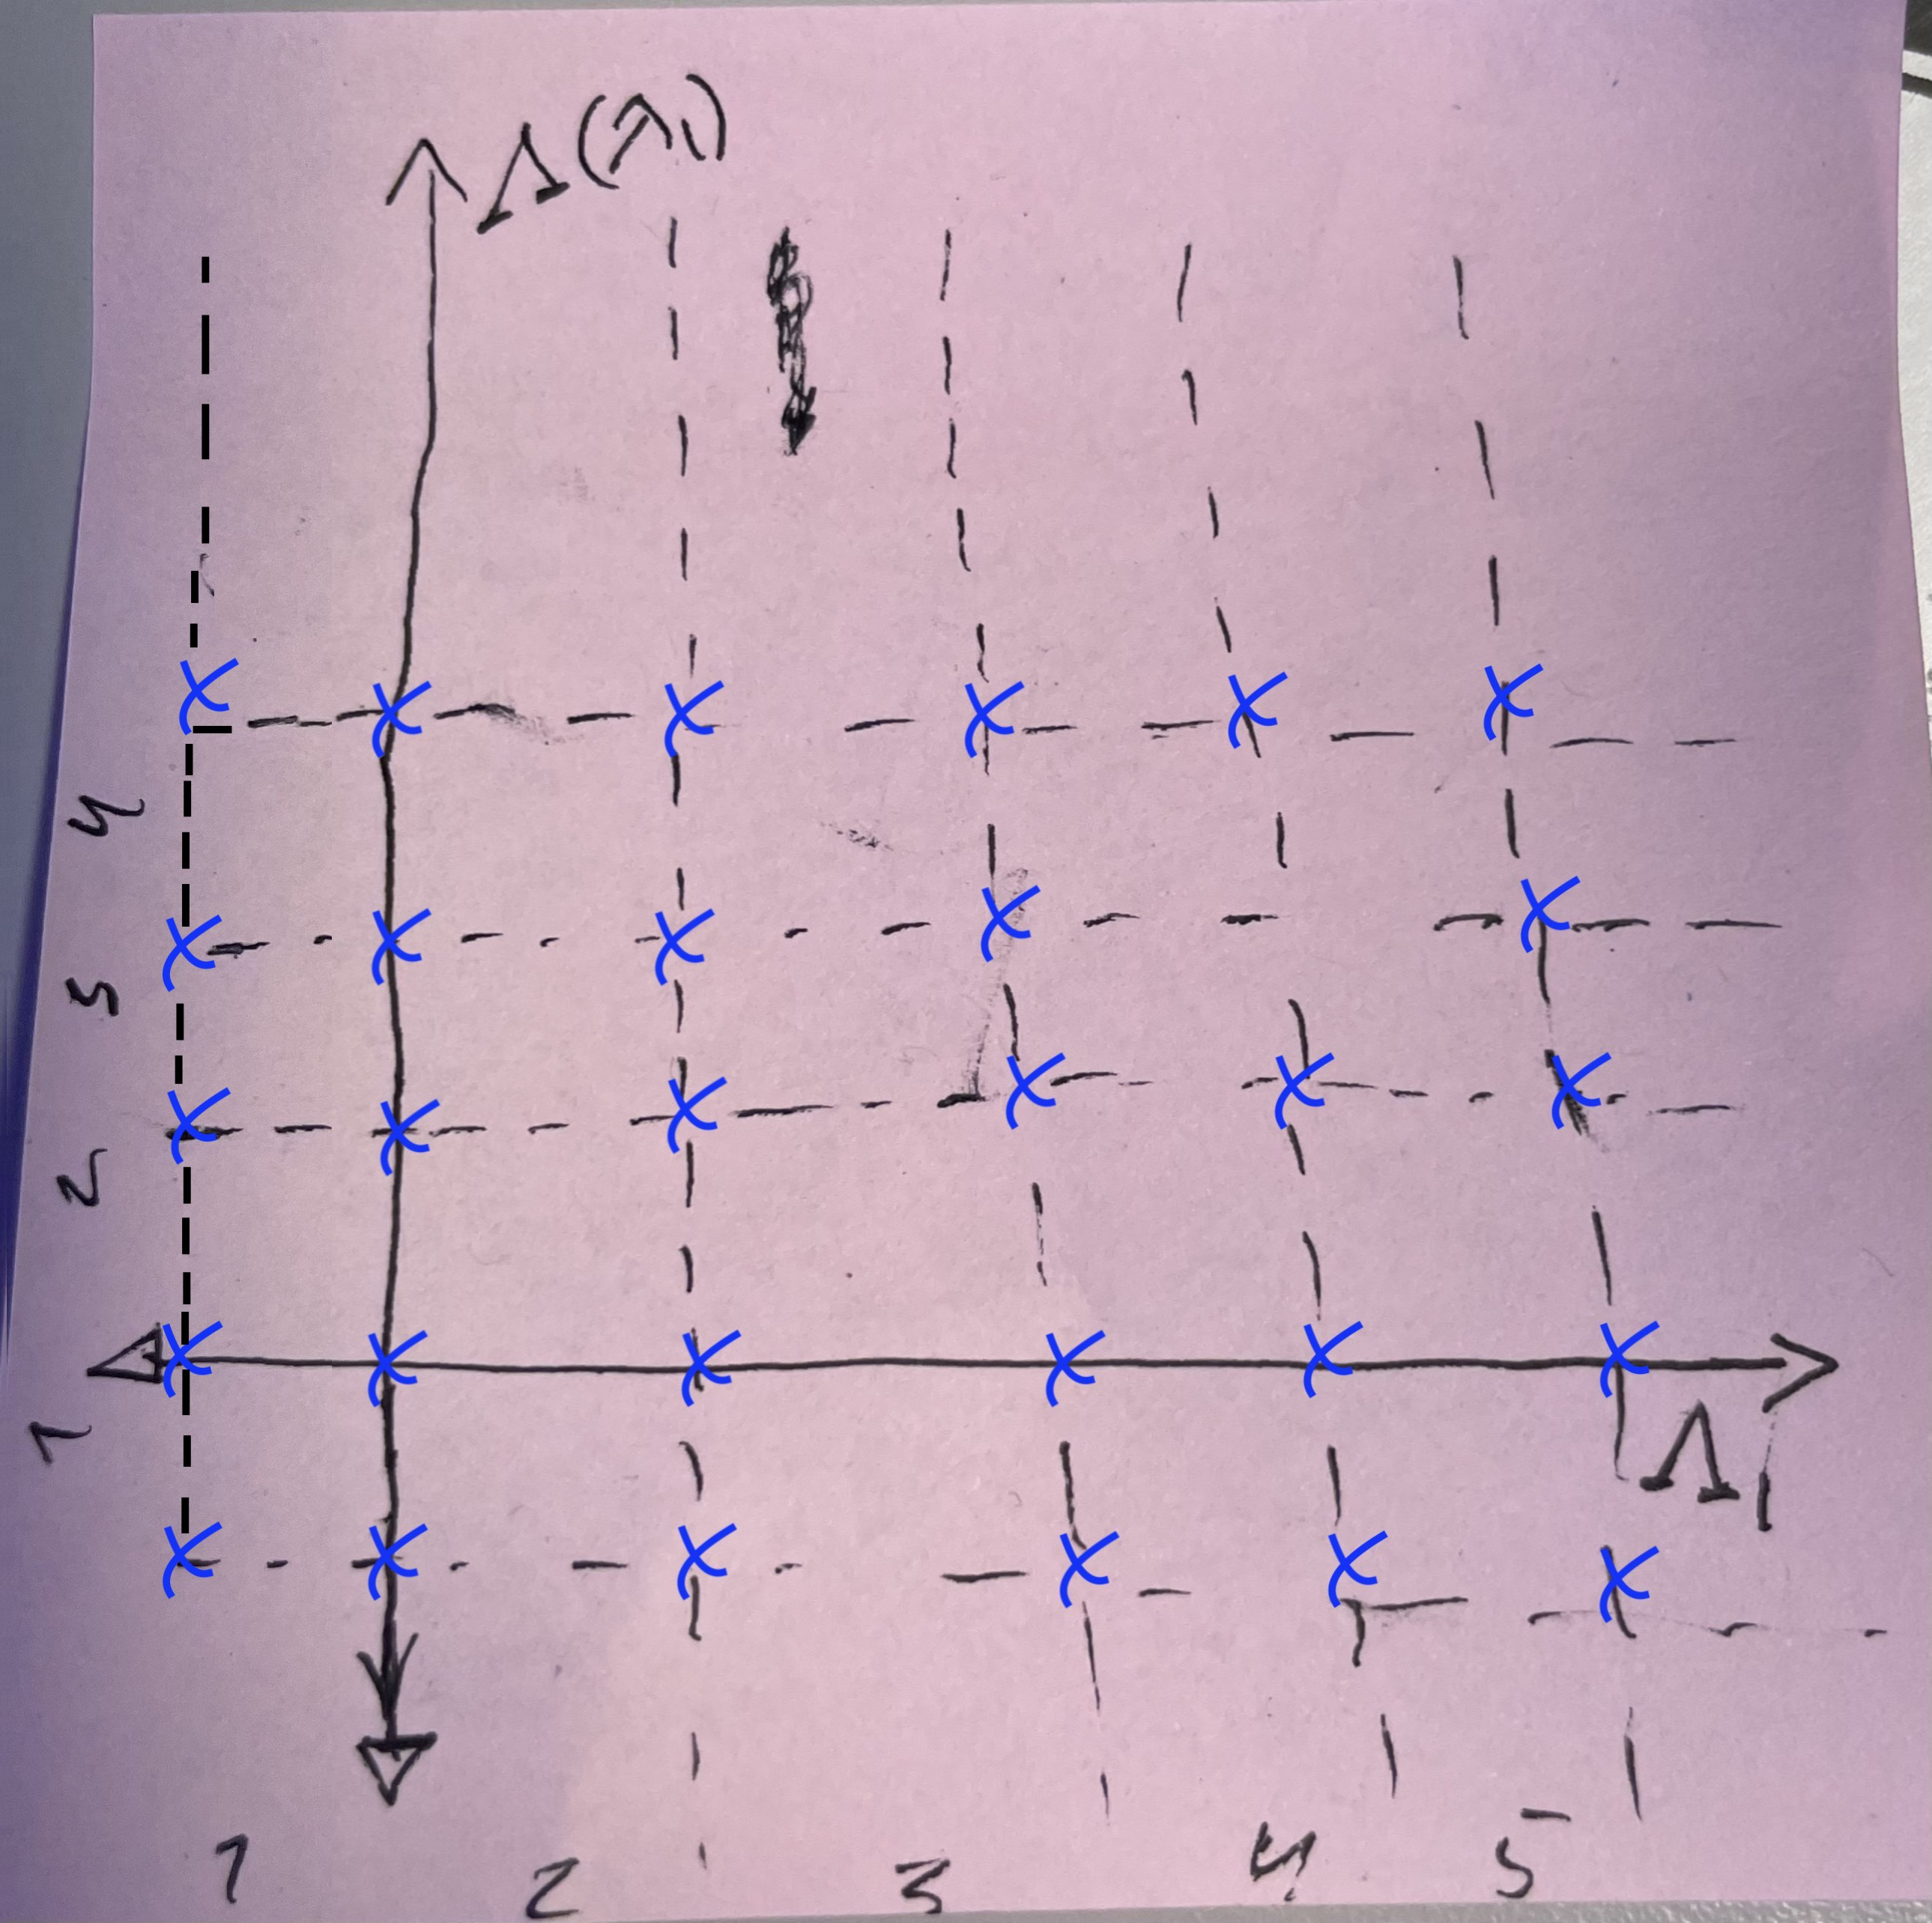
\includegraphics[width=0.9\linewidth]{spec_no_shift.jpg}
        %* Figure 1              
        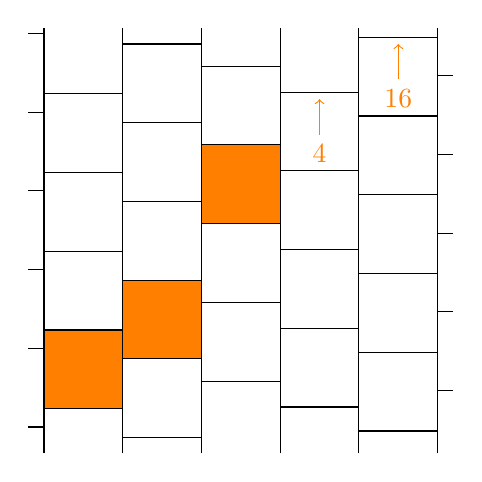
\begin{tikzpicture}[scale=1]
            % Define the tile
            \def\tile{
            % Draw the unit square
            \draw[fill=white] (0,0) rectangle (1,1);
            }
            \def\tiletwo{
            %\draw[fill=gray!65] (0,0) rectangle (1,1);
            \draw[fill=orange] (0,0) rectangle (1,1);
            %\draw[->] (0.5,0) -- (0.5,0.9);  % If arrows from the middle
            }
            % Right border tile
            \def\tileThree{
            %\draw[fill=red] (0,0) rectangle (1,1);  % test tile to se if we got the right one
            \draw[black] (0,1) -- (0+0.2,1);  % Right_top
            \draw[black] (0,0) -- (0+0.2,0);  % Right_bottom
            }
            % Left border tile
            \def\tileFour{
            % If using test square, must change from x=0 to x=1 for the left border markers
            %\draw[fill=red] (0,0) rectangle (1,1);  % test tile to se if we got the right one
            \draw[black] (0,1) -- (0-0.2,1);  % Right_top
            \draw[black] (0,0) -- (0-0.2,0);  % Right_bottom
            }
            
            % Exponential function parameters
            \pgfmathsetmacro{\base}{2} % Base of the exponential function
            \pgfmathsetmacro{\expMinTwo}{exp(-2)}
            \pgfmathsetmacro{\expMinOne}{exp(-1)}
            \pgfmathsetmacro{\expZero}{exp(0)}
            \pgfmathsetmacro{\expOne}{exp(1)}
            \pgfmathsetmacro{\expTwo}{exp(2)}
            \pgfmathsetmacro{\expThree}{exp(3)}
            \pgfmathsetmacro{\expFour}{exp(4)}

            % Shift list
            \def\BetaMinOne{\expMinOne}
            \def\BetaZero{\expZero}
            \def\BetaOne{\expOne}
            \def\BetaTwo{\expTwo}
            \def\BetaThree{\expThree}
            \def\BetaFour{\expFour}

            % Left border markers
            \foreach \x in {0}{
                \foreach \y in {0,1,2,3,4}{
                    \pgfmathsetmacro{\shiftX}{\x}
                    \pgfmathsetmacro{\shiftY}{\y + \expMinTwo}
                    \pgfmathsetmacro{\shiftSingle}{\expMinTwo}
                    
                    % Drawing the rest of the middle cubes
                    \begin{scope}[shift={(\shiftX,\shiftY)}]
                        \tileFour
                    \end{scope}
        }}
            % Right border markers
            \foreach \x in {5}{
                \foreach \y in {-54,...,-51}{
                    \pgfmathsetmacro{\shiftX}{\x}
                    \pgfmathsetmacro{\shiftY}{\y + \BetaFour}
                    \pgfmathsetmacro{\shiftSingle}{\BetaFour}
                    % Drawing the rest of the middle cubes
                    \begin{scope}[shift={(\shiftX,\shiftY)}]
                        \tileThree
                    \end{scope}
                    
        }}


            % Draw the tiling pattern Latter part
            \foreach \x in {1}{
                \foreach \y in {-1,...,3}{
                    \pgfmathsetmacro{\shiftX}{\x}
                    \pgfmathsetmacro{\shiftY}{\y + \BetaZero}
                    \pgfmathsetmacro{\shiftSingle}{\BetaZero}
                    % Drawing the rest of the middle cubes
                    \begin{scope}[shift={(\shiftX,\shiftY)}]
                        \tile
                    \end{scope}
                    % No need for orange cubes as they would be outside
                }}
            \foreach \x in {2}{
                \foreach \y in {-2,...,1}{
                    \pgfmathsetmacro{\shiftX}{\x} 
                    \pgfmathsetmacro{\shiftY}{\y + \BetaOne} 
                    \pgfmathsetmacro{\shiftSingle}{0+\BetaOne}
                    % Drawing the rest of the middle cubes
                    \begin{scope}[shift={(\shiftX,\shiftY)}]
                        \tile
                    \end{scope}
                    % No need for orange cubes as they would be outside
                }}
            \foreach \x in {3}{
                \foreach \y in {-7,...,-4}{
                    \pgfmathsetmacro{\shiftX}{\x}
                    \pgfmathsetmacro{\shiftY}{\y + \BetaTwo}
                    \pgfmathsetmacro{\shiftSingle}{\BetaTwo}
                    % Drawing the rest of the middle cubes
                    \begin{scope}[shift={(\shiftX,\shiftY)}]
                        \tile
                    \end{scope}
                    % No need for orange cubes as they would be outside
                    % REMEMBER that we have shifted the entirety of what is plotted from this column, 
                    % our grid is still x: -1,...,5 and   y: 0,...,4 i.e., The leftmost markers!!                  
                    \ifnum\y=-4
                        \draw[->, orange] (\x+0.5,3.85) node[below] {$4$} -- (\x+0.5,4.3);
                    \fi
                }}
                \foreach \x in {4}{
                    \foreach \y in {-20,...,-16}{
                    \pgfmathsetmacro{\shiftX}{\x}
                    \pgfmathsetmacro{\shiftY}{\y + \BetaThree}
                    \pgfmathsetmacro{\shiftSingle}{\BetaThree}
                    % Drawing the rest of the middle cubes
                    \begin{scope}[shift={(\shiftX,\shiftY)}]
                        \tile
                    \end{scope}
                    % No need for orange cubes as they would be outside
                    % REMEMBER that we have shifted the entirety of what is plotted from this column, 
                    % our grid is still x: -1,...,5 and   y: 0,...,4 i.e., The leftmost markers!!               
                    \ifnum\y=-16
                        \draw[->, orange] (\x+0.5,4.55) node[below] {$16$} -- (\x+0.5,5);
                    \fi
                }}
                
            % Draw the tiling pattern
            \foreach \x in {0}{
                \foreach \y in {0,1,2,3}{
                    \pgfmathsetmacro{\shiftX}{\x}
                    \pgfmathsetmacro{\shiftY}{\y + \BetaMinOne}
                    \pgfmathsetmacro{\shiftSingle}{0+\BetaMinOne}
                    % Drawing the rest of the middle cubes
                    \begin{scope}[shift={(\shiftX,\shiftY)}]
                        \tile
                    \end{scope}
                }  
            }
            
            % Orange cube overlay
            \foreach \x in {0,1,2}{
                \foreach \y in {0,1,2,3}{
                    \ifnum\x=0
                        \pgfmathsetmacro{\shiftX}{\x}
                        \pgfmathsetmacro{\shiftY}{\y + \BetaMinOne}
                        \pgfmathsetmacro{\shiftSingle}{0+\BetaMinOne}
                    \fi
                    \ifnum\x=1
                        \pgfmathsetmacro{\shiftX}{\x}
                        \pgfmathsetmacro{\shiftY}{\y + \BetaZero}
                        \pgfmathsetmacro{\shiftSingle}{0+\BetaZero}
                    \fi
                    \ifnum\x=2
                        \pgfmathsetmacro{\shiftX}{\x}
                        \pgfmathsetmacro{\shiftY}{\y + \BetaOne}
                        \pgfmathsetmacro{\shiftSingle}{0+\BetaOne}
                    \fi
                    % Drawing a new line of shifted colored cubes on top at the first row
                    \ifnum\y=0
                        \begin{scope}[shift={(\shiftX,\shiftY)}]
                            \tiletwo
                        \end{scope}
                    \fi
        }}
            % get the outline grid 
            % Whole black lines
            \foreach \x in {0,1,2,3,4,5}{
                \draw (\x,0-0.2) -- (\x,5+0.2);  % Shift only in the vertical direction, therefore only one line
            }
        \end{tikzpicture}
        %* —————————————————
        \caption{Non-periodic tiling of unit cubes}
        \label{fig:tiling_eight}
    \end{subfigure}
    \caption{Illustrated in \cref{fig:tiling_seven} is a clique of size $2^8=256$ in the Keller graph of $G_{8,2}$, which disproves Keller's conjecture for $d\geq8$. Each grey square of $8$ dots represents a vertex, and each dot inside the square represents a coordinate. The coordinate set in the Keller graph of $G_{8,2}$ is $\braq{0,1,2,3}$, where the colors black, dark blue, white, or light blue respectively represents each of the possible coordinate values. Observe that for the vertices to be adjacent, it is enough for any two vertices to have a complimentary dot, which means either black versus white or dark blue versus light blue; \textsc{and} at least one dot of a different color as a different color represents a different coordinate. Illustrated in \cref{fig:tiling_eight} is a non-periodic tiling of $\R^2$ where the $n$'th column of unit cubes is shifted in the vertical direction by the value of $e^n$, for all $n\in\Z$. The arrow with an orange number indicates the number of unit squares from the arrow to the orange-colored unit square. If this were a lattice tiling, all orange-colored squares would be on the same horizontal line. The lines of the $-2$'th and $4$'th columns of unit cubes can be observed at the left and right edges, respectively.}
    \label{fig:tilings_seven_eight}
\end{figure}

In addition to the tilings related to Keller's \namecref{conj:keller_tiling}, periodicity is another essential concept. A monohedral tiling is \emph{non-periodic} if it admits no period parallelograms \cite{penrosePentaplexityClassNonPeriodic1979}, and \emph{vice versa}. In our case, this intuitively means that if we know the arrangement of the tile with respect to its vertices and edges within a parallelogram, then we can construct the entire tiling by repeating this arrangement. That is, repeating the parallelogram, not the tile. We refer to \cite[p.29-30]{grunbaumTilingsPatterns1987} for an in-depth explanation with great images. Nevertheless, if our tile only tiles non-periodically, then we say it is \emph{aperiodic}. That is, \emph{every} tiling possible with the tile is non-periodic and must necessarily be so \cite[p. 520]{grunbaumTilingsPatterns1987}. Authors of \cite{grunbaumTilingsPatterns1987} stressed this fact in $1987$, and still, there seems to be confusion between the terms \emph{non-periodic} and \emph{aperiodic}, which is why we stress this again\footnote[1]{As will be explained, the terms are confused in \cite{lagariasOrthonormalBasesExponentials2000,liuUniformityNonUniformGabor2003}}.

In higher dimensions, the unit cube can also tile non-periodically. Two simple examples are illustrated in \cref{fig:single_shift_horizontal_tiling,fig:single_shift_vertical_tiling}. Try creating a single parallelogram that can be used to tile the entire plane, and one will quickly see that this cannot be done. However, one can consider them to be \emph{half-periodic}, in the sense that they do not admit a vertical or horizontal period, respectively, but do allow for a period in the same direction as the shift. That is a horizontal and vertical period, respectively \cite{kolountzakisTilingsTranslation2010}. To create a completely non-periodic tiling in dimension $2$, one can shift the $n$'th column of unit cubes in the vertical direction with $e^n$, for all $n\in\Z$ \cite{liuUniformityNonUniformGabor2003}. This is illustrated in \cref{fig:tiling_eight}, and is significant because it shows that the unit cube can tile non-periodically in all $d\geq 2$. However, as the unit cube can always be organized into a lattice and hence tile periodically, it is not an aperiodic tiling.
\begin{remark}
    Nevertheless, by arranging unit cubes into a \emph{new} tile, one can get an aperiodic tiling for all $d\geq3$, as done in \cite{lagariasKellerCubetilingConjecture1992}. (Max: Given that it is actually true that this organization/new tile/ of unit cubes EXCLUSIVELY tiles non-periodically. Not known to me yet). The fact that the new tile only consists of unit cubes in a particular arrangement is not equivalent to the statement that there \emph{are} aperiodic cube tilings in all $d\geq3$ as stated in \cite{lagariasOrthonormalBasesExponentials2000,liuUniformityNonUniformGabor2003}, as one considers a tiling which, in fact, is \textsc{not} a cube, only consisting of cubes; and by the very definition of aperiodicity means that it must exclusively tile non-periodically, which \emph{cube tilings} intrinsically do not as highlighted above. Furthermore, \cite{lagariasOrthonormalBasesExponentials2000} provides no source for this "well-known" statement, and \cite{liuUniformityNonUniformGabor2003} makes a reference to \cite{lagariasKellerCubetilingConjecture1992}, but the explanation here is both insufficient and unclear, as this result is \textsc{never} stated anywhere. (Max: If I am wrong with this, then I cannot read. This can very well be the case when it comes to math, but I am pretty certain of this latter sentence. It can be true that the result is implied by the paper or somehow obvious in a way I cannot understand, but that is not a clear and sufficient statement of the result from my undergraduate perspective.)
\end{remark}

It is precisely the higher dimensional tilings that either or both are non-periodic and that counterexample Keller's \namecref{conj:keller_tiling} that we intuitively define to be the exotic and counterintuitive tilings.

%* ———————————————————————————— Tilings ——————————————————
%* Here, in the definitions of tiling, we allow the distinct translations of the domain to overlap on sets of measure zero rather than the traditional condition of empty overlap.
%- Now, in defining a tiling more formally, one possible approach is to define it as a non-overlapping covering of the space.

Now, we endeavor to establish a more rigorous definition of tiling. One possible approach is to define it as a non-overlapping covering of the space. By this, we mean that a subset $\Omega \subset \R^d$ of non-zero measure is a tile, and a set $\Lambda \subset \R^d$ is a tiling set if they satisfy both of the following conditions. First, $\Omega+\lambda$ for $\lambda \in \Lambda$ must cover $\R^d$ up to measure zero. Secondly, all intersections $(\Omega+\lambda) \cap (\Omega+\lambda')$ of distinct elements $\lambda,\lambda' \in \Lambda$ must have measure zero. Note that $\Omega+\lambda$ denotes the translate of $\Omega$ by the vector $\lambda$. However, instead of the more intuitive geometric definition, we use the following as our working \namecref{def:tiling} in terms of indicator functions \cite{kolountzakisTilingsTranslation2010,kolountzakisStructureTilingsLine1996}.  % - However, instead of the more intuitive geometric definition, we use the following as our working definition in terms of indicator functions \cite{kolountzakisTilingsTranslation2010,kolountzakisStructureTilingsLine1996}.
% - More formally/Nevertheless, tilings can also be expressed using indicator functions as follows \cite{kolountzakisTilingsTranslation2010}. \SigridChange{/} We will, however, define tilings in terms of indicator functions as follows \cite{kolountzakisTilingsTranslation2010} \cite{kolountzakisStructureTilingsLine1996}.
% - Rather than defining tiling in terms of a non-overlapping covering of the space, we will instead define tiling by the indicator function, using little of our geometric intuition \cite{kolountzakisTilingsTranslation2010} \cite{kolountzakisStudyTranslationalTiling2003}. 
\begin{definition}[Tiling set]\label{def:tiling}
    Let $\Omega \subset \R^d$ be a subset with non-zero measure, and consider a discrete set $\Lambda \subset \R^d$. If
    \begin{equation}\label{eq:tiling_set}
        \sum_{\lambda \in \Lambda} \indicator{\Omega}{x-\lambda} = 1, \quad a.e. \text{\space\space} x \in \R^d.
    \end{equation}
    then $\Omega$ is called a \emph{tile}, and $\Lambda$ is called a \emph{tiling set} for $\Omega$. We say that $(\Omega, \Lambda)$ is a \emph{tiling pair}.
\end{definition}
\begin{remark}
    We can also say that $\Omega$ \emph{tiles $\R^d$ by translation}, or that $\Omega$ is a \emph{tiling} of $\R^d$. 
\end{remark}
\begin{remark}
    Additionally, one can define tilings more generally. By this, we mean that in place of the indicator function, we can have a non-negative, integrable function $f$. Other than allowing for any other constant value than $1$, the definition is the same. The reader is referred to \cite{kolountzakisTilingsTranslation2010,kolountzakisStructureTilingsLine1996} for more details on this topic.
\end{remark}
% Direct in text:
% In other words, we can also say that $\Omega$ \emph{tiles $\R^d$ by translation}, or that $\Omega$ is a \emph{tiling} of $\R^d$. Additionally, one can define tilings more generally. By this, we mean that in place of the indicator function, we can have a non-negative, integrable function $f$. Other than allowing for any other constant value than $1$, the definition is the same. Note that we still require the same constant value almost everywhere. The reader is referred to \cite{kolountzakisTilingsTranslation2010} for more details on this topic.
%* ———————————————————————————— One dimension  ——————————————————
%* Viktig, må inn en bit her om 
%* som en konsekvens av Kellers theorem så får vi nå akkurat den samme formen på disse tilings settene 
%* de må ligge inneholt i akkurat de samme typene mengder, og de kan ikke være ekte mindre for da får vi ikke oppfylt tiling kravet mitt.
If we now restrict our attention to tilings of the unit cube in $\R^d$, Keller's \namecref{thrm:keller_tiling} immediately gives the following for dimension one.  For $d=1$, the unit cube is simply the unit interval $I = \bras{0,1}$. %In dimension one, the unit cube is simply the unit interval $I = \bras{0,1}$. 

\begin{lemma}\label{lem:tiling_unit_1d}
    %The set $\Lambda = \Z +\alpha$ for some value $\alpha\in \R$ constitutes a tiling set for $I$.
    %The only subsets $\Lambda \in \R$ such that $\Lambda$ is a tiling set for $I$ are $\Lambda = \Z +\alpha$ for some value $\alpha\in \R$.
    The only subsets $\Lambda \in \R$ such that $\Lambda$ is a tiling set for $I$ are the translates $\Lambda = \Z +\alpha$ for a fixed value $\alpha\in \R$. 
\end{lemma}

\begin{proof}  % This follows directly from \cref{thrm:keller_tiling}. Take $\lambda, \lambda' \in \Lambda$. 
    %  Må konkret gå tilbake til definisjonen du har valgt. For den kan vi bruke eksplisitt til å si:
    %Det Keller's theorem forteller meg, er at jeg må ha noe som er en undermengde av $\Lambda = \Z + \alpha$, og i og med at jeg må ha 1 almost everywhere, så gjør det at hvis jeg tar bort et punkt fra $\Lambda$ slik at vi har $\Lambda \subset \Z + \alpha$, så vil jeg få et intervall hvor jeg har 0.
    %  La oss nå si at et punkt er utelatt. Det betyr at $\sum \indicator{\Omega}{t} = 0$ og vi kan si nøyaktig hvor det er null, for det er på det punktet vi har utelatt. Dvs, $x\in I+\lambda'$, hvor $\lambda'$ er punktet vi utelot fra flisleggingsmengden. Videre, så er målet av $I+\lambda'$ positivt, det er ikke neglisjerbart. Dvs, der du ikke har verdien 1, de områdene, de er ikke neglisjerbare. Og videre vet vi at vi har $x\in I+\lambda'$, dvs et helt slikt interval, hvor $\sum \indicator{\Omega}{t} = 0$, og dette området har positivt mål. 
    Let $\Lambda \subset \R^d$. Using Keller's \namecref{thrm:keller_tiling}, \cref{thrm:keller_tiling}, we instantly get that there must be an integer distance between two distinct points $\lambda,\lambda' \in \Lambda$ if $\Lambda$ is to be a tiling set for $I$. Hence, we know that $\Lambda \subseteq \Z +\alpha$ for a fixed $\alpha\in \R$. Now, given an arbitrary point $\lambda' \in \Z +\alpha$, assume that $\lambda'\notin \Lambda$ so that we have a case where $\Lambda \subset \Z+\alpha$. However, by using \cref{def:tiling}, observe now that we have an entire interval, specifically $I+\lambda'$, where $\indicator{I}{x - \lambda'} = 0$. As $\mes{I+\lambda'} = 1 $, this is non-negligible, and we do not achieve
    \begin{equation*}
        \sum_{\lambda \in \Lambda\setminus \braq{\lambda'}} \indicator{I}{x-\lambda} = 1, \quad a.e. \text{\space\space} x \in \R^d.
    \end{equation*}
    %* As $\mes{I+\lambda'} = 1 $, this is non-negligible, and we do not achieve $\indicator{I}{x-\lambda} = 1$ almost everywhere for $x\in\R^d$ with the set $\Lambda\setminus \braq{\lambda'}$. % In short: That is, we have a non-negligible region with a value not equal to one.
    Hence $\lambda' \in \Lambda$, which shows that $\Lambda = \Z+\alpha$. This concludes the proof that there are no other tiling sets for $I$ in dimension $d=1$. %and that $\Lambda$ is a tiling set for $I$ . %for a tiling set $\Lambda$ of
\end{proof}

Increasing the dimension by one, we get more flexibility. In particular, when $d=2$, we do not necessarily need to have a lattice tiling as the one in \cref{fig:tiling_one}. We can have tilings where we translate single or multiple \emph{columns} of the unit cube, shown in \cref{fig:single_shift_vertical_tiling,fig:multiple_shift_vertical_tiling}; or single or multiple \emph{rows} of the unit cube, shown in \cref{fig:single_shift_horizontal_tiling,fig:multiple_shift_horizontal_tiling}. We will see later in \cref{chap:equivalence} that \cref{fig:tiling_figures} to some extent fully captures the flexibility of two dimensions. We remark that all \cref{fig:single_shift_vertical_tiling,fig:multiple_shift_vertical_tiling,fig:single_shift_horizontal_tiling,fig:multiple_shift_horizontal_tiling} clearly illustrates that all tilings of the unit cube in $\R^2$ also satisfy Keller's \namecref{thrm:keller_tiling}. 




\begin{figure}[t!]%h!
    \centering
    \begin{subfigure}{.47\textwidth}
        \centering
        %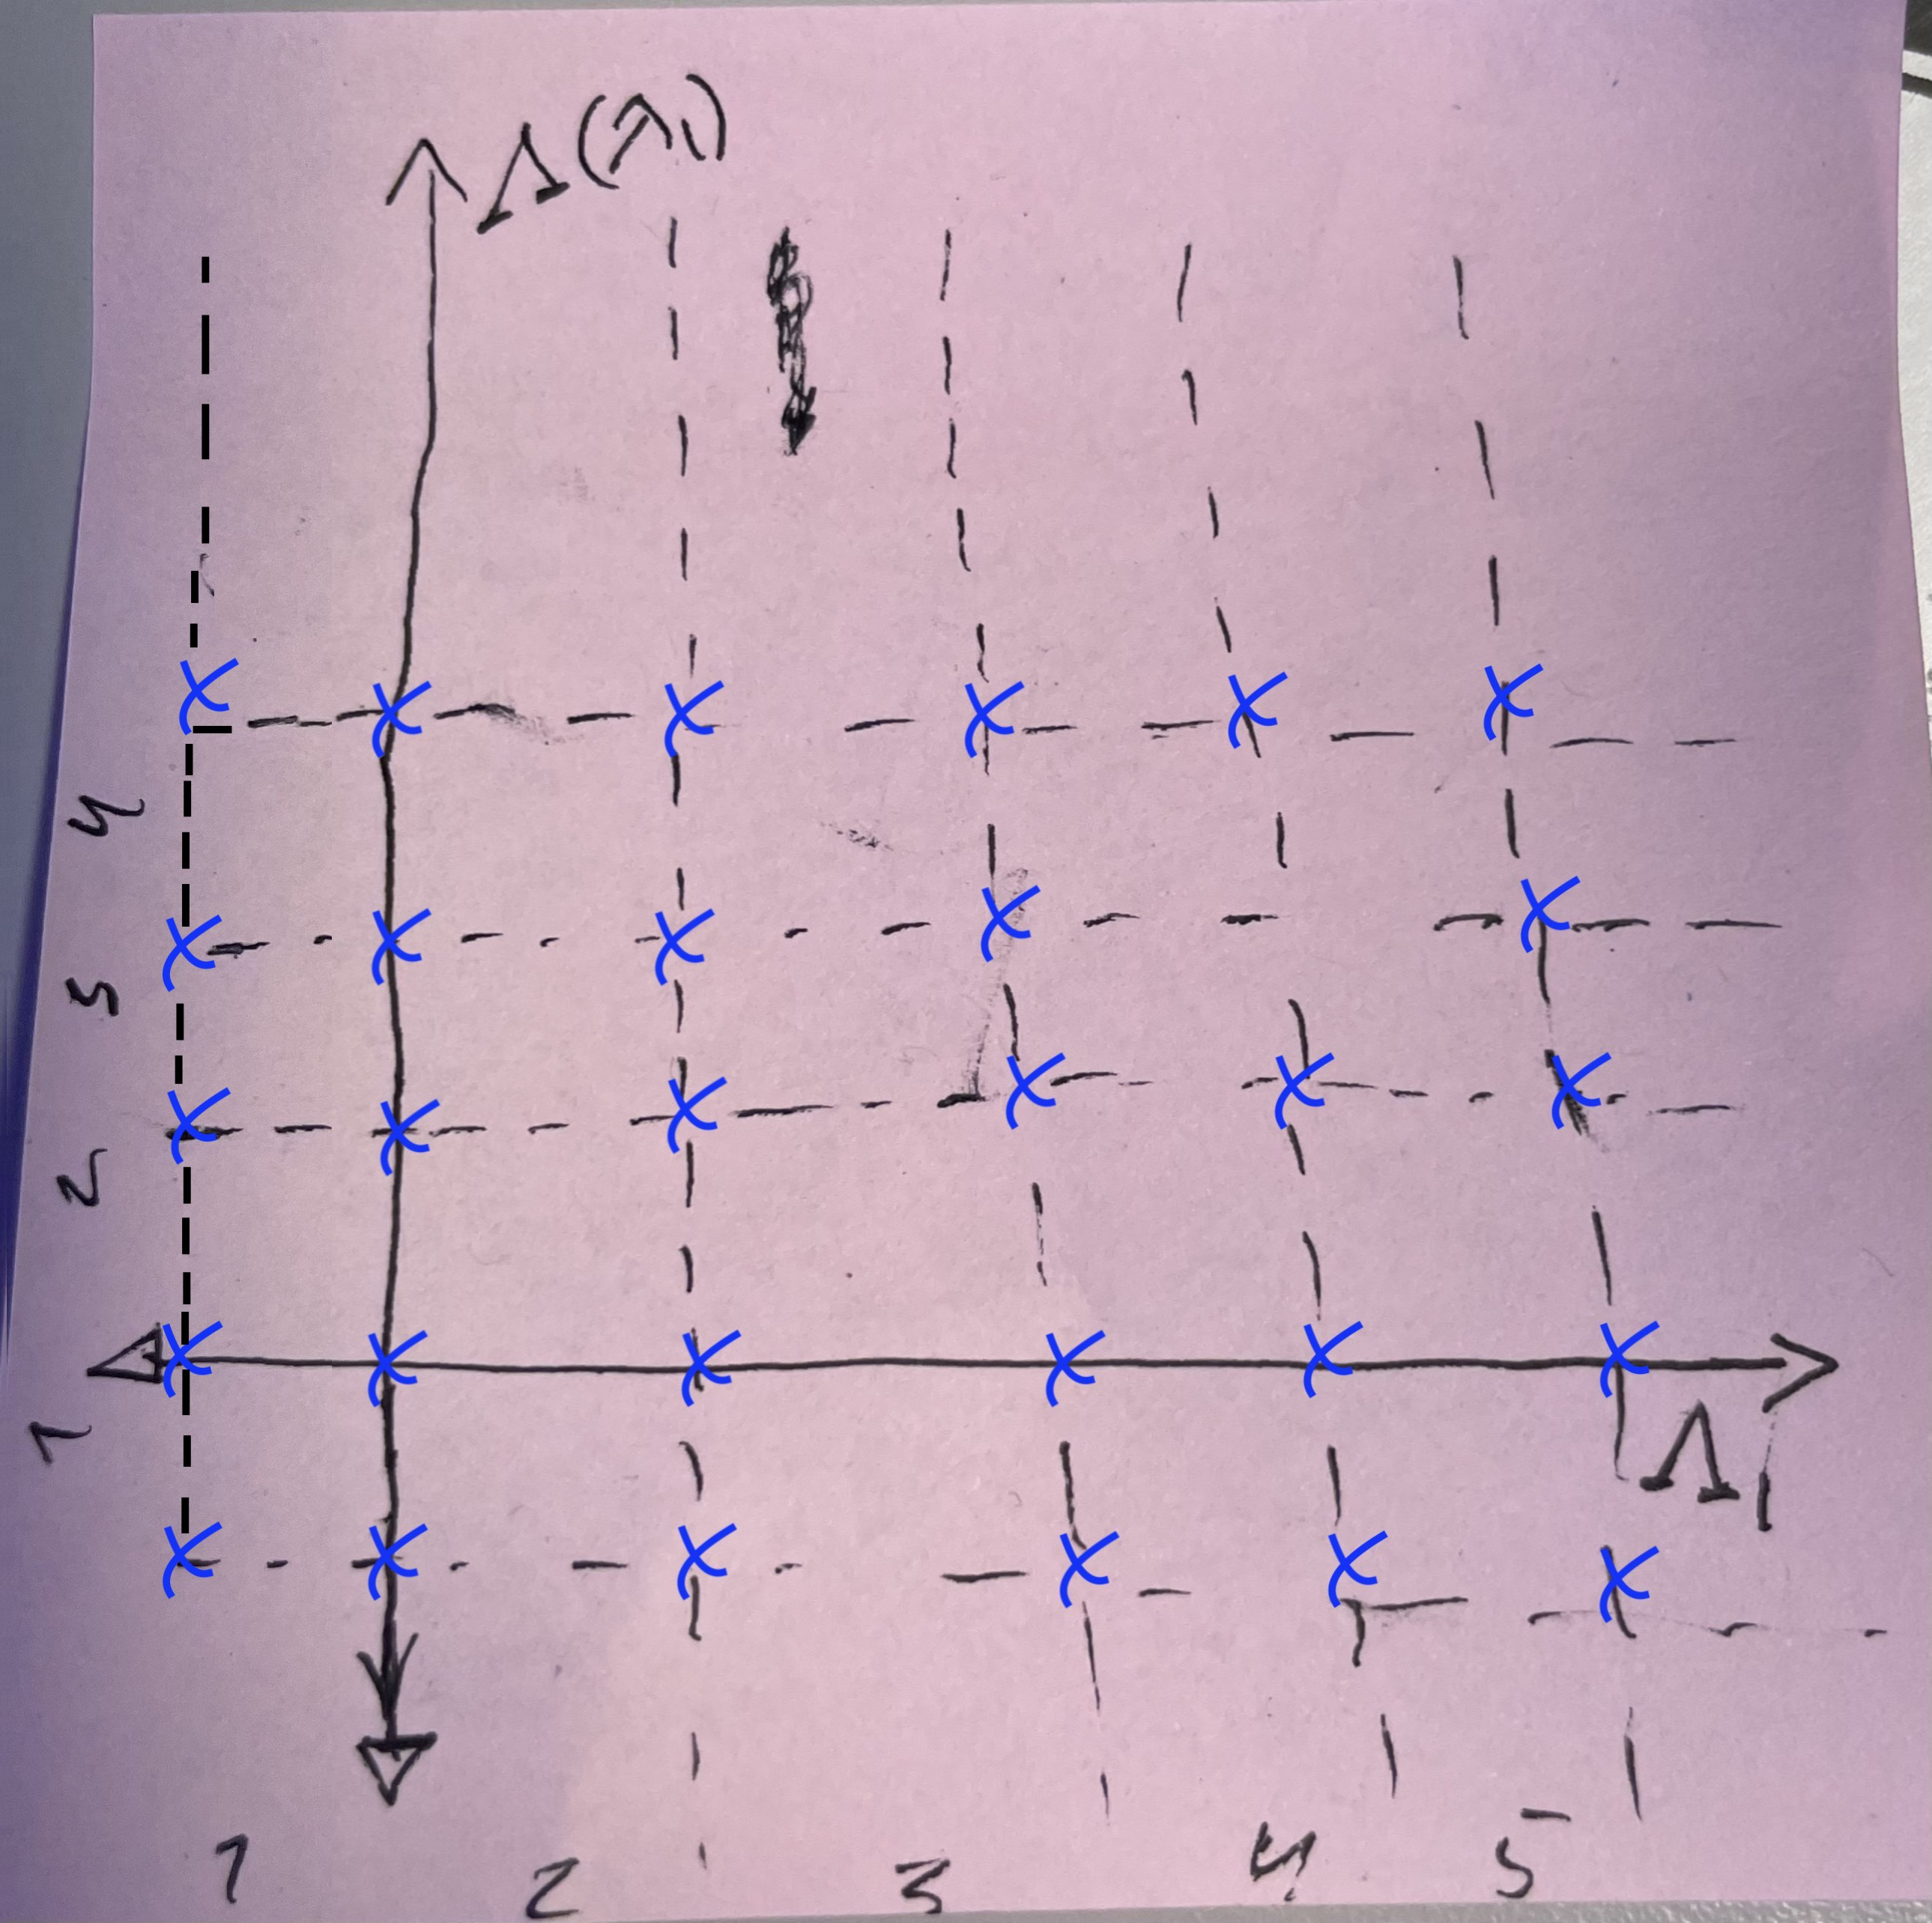
\includegraphics[width=0.9\linewidth]{spec_no_shift.jpg}
        %* Figure 1
        \begin{tikzpicture}[scale=1]
            % Define the tile
            \def\tile{
            \draw[fill=white] (0,0) rectangle (1,1);
            }
            \def\tiletwo{
            %\draw[black, fill=gray!65] (0,0) rectangle (1,1);
            %\draw[black, fill=cyan!65] (0,0) rectangle (1,1);
            \draw[pattern=north east lines, pattern color=MaxCyan4] (0,0) rectangle (1,1);
            }
            
            % Draw the tiling pattern
            % Shifted line, part 1, left and right half tiles 
            \foreach \x in {0}{
                %\draw[cyan, fill=cyan] (\x-0.2,2) rectangle (\x+0.5,3);  % leftmost value to the first square
                \draw[white, pattern=north east lines, pattern color=MaxCyan4] (\x-0.2,2) rectangle (\x+0.5,3); % leftmost value to the first square
            }
            \foreach \x in {6}{
                \draw[white, pattern=north east lines, pattern color=MaxCyan4] (\x+0.2,2) rectangle (\x-0.5,3);
                %\draw[gray!65, fill=cyan!65] (\x+0.2,2) rectangle (\x-0.5,3);  % rightmost value to the last square
            }
            % part 2, whole tiles in the middle
            % must be after the above code in order to get black lines at the correct spots
            \foreach \y in {2}{
                \foreach \x in {0,1,2,3,4}{
                    \pgfmathsetmacro{\shiftX}{\x+0.5} % Set horizontal shift
                    \pgfmathsetmacro{\shiftY}{\y}
                    \begin{scope}[shift={(\shiftX,\shiftY)}]
                        \tiletwo
                    \end{scope}
                }
            }
            % Everything else
            \foreach \y in {0,1,3,4}{
                \foreach \x in {0,1,2,3,4,5}{
                    \pgfmathsetmacro{\shiftX}{\x} % Set horizontal shift
                    \pgfmathsetmacro{\shiftY}{\y}
                    \begin{scope}[shift={(\shiftX,\shiftY)}]
                        \tile
                    \end{scope}
                }
            }
            % get the outline grid 
            



% small black lines at the left and right
\foreach \y in {0,1,2,3,4,5}{
    \draw (0-0.2,\y) -- (0,\y);  % Left
    \draw (6,\y) -- (6+0.2,\y);  % Right
    
}

% small black lines at the top and bottom
\foreach \x in {0,1,2,3,4,5,6}{
    \draw (\x,0-0.2) -- (\x,0);  % Top
    \draw (\x,5) -- (\x,5+0.2);  % Bottom
}
        \end{tikzpicture}
        %* —————————————————
        \caption{Single row shift}
        \label{fig:single_shift_horizontal_tiling}
    \end{subfigure}\quad
    \begin{subfigure}{.47\textwidth}
        \centering
        %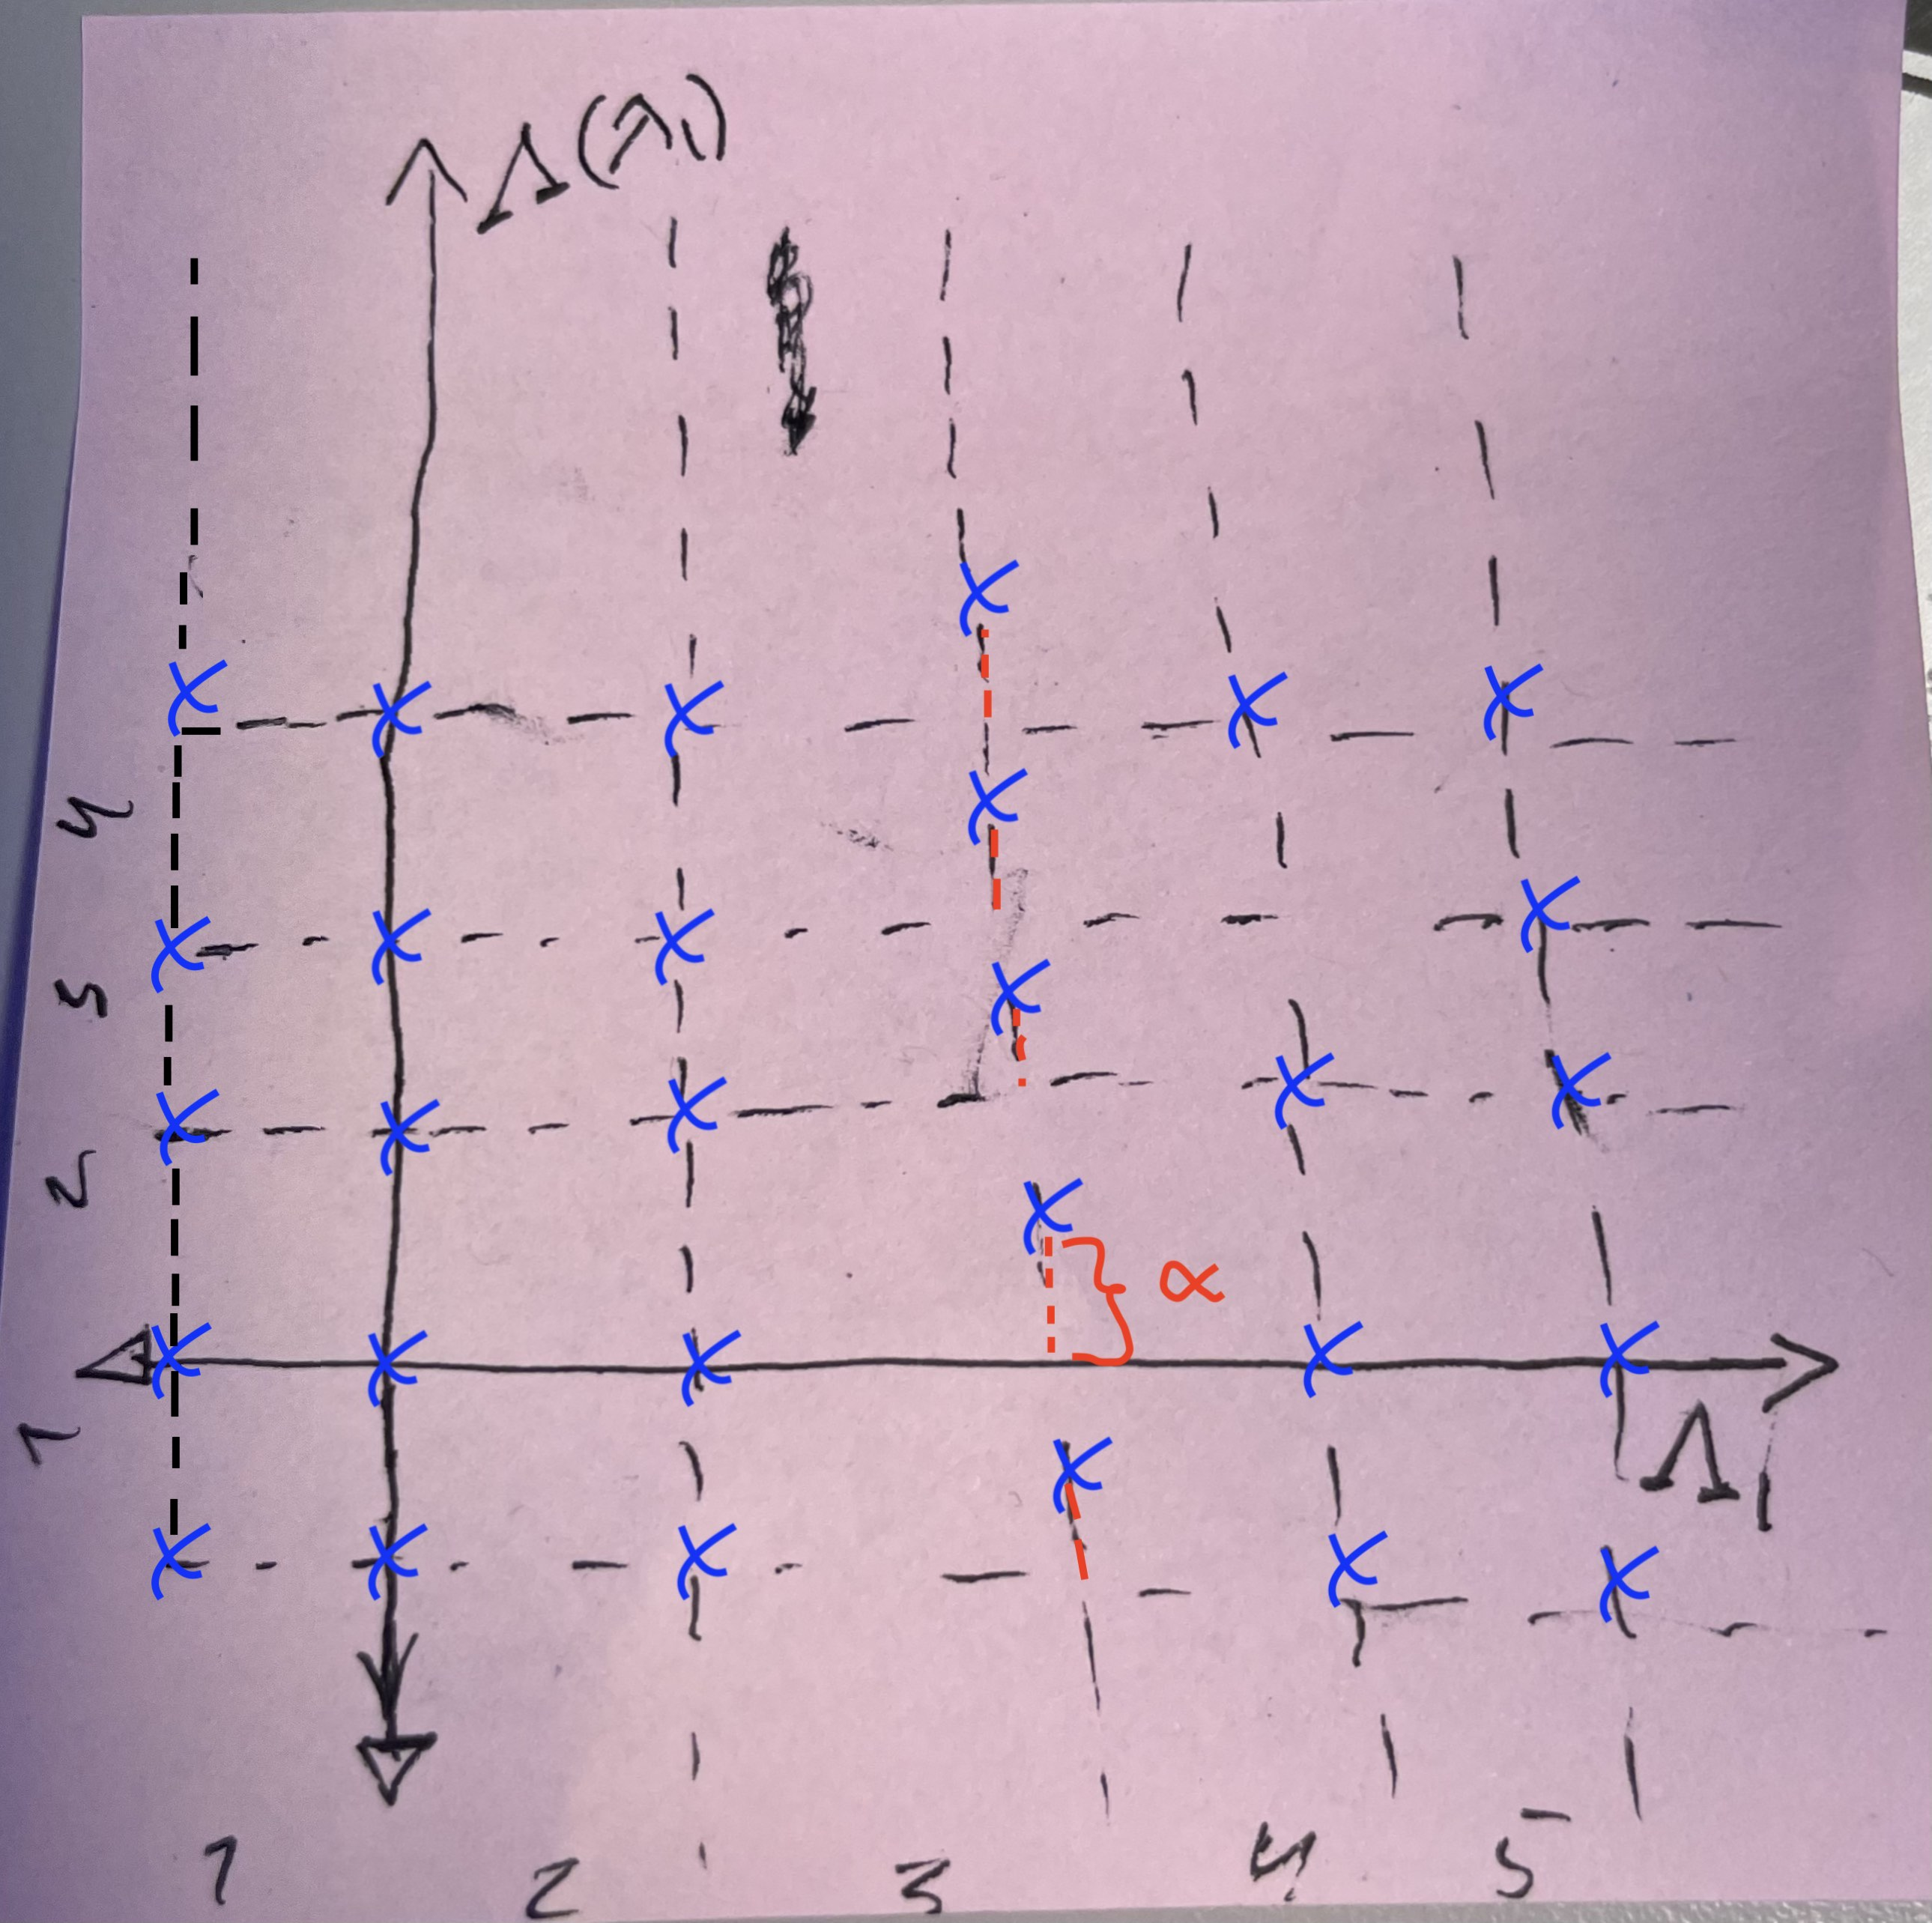
\includegraphics[width=0.9\linewidth]{spec_single_shift.jpg}
        %* Figure 2
        \begin{tikzpicture}[scale=1]
            % Define the tile
            \def\tile{
            \draw[fill=white] (0,0) rectangle (1,1);
            }
            \def\tiletwo{
            %\draw[fill=gray!65] (0,0) rectangle (1,1);
            %\draw[fill=YellowOrange] (0,0) rectangle (1,1);
            \draw[pattern=north east lines, pattern color=MaxOrange] (0,0) rectangle (1,1);
            }
            
            % Draw the tiling pattern
            % Shifted line, part 1, left and right half tiles 
            \foreach \y in {0}{
                %\draw[YellowOrange, fill=YellowOrange] (2,\y-0.2) rectangle (3,\y+0.5);
                \draw[white, pattern=north east lines, pattern color=MaxOrange] (2,\y-0.2) rectangle (3,\y+0.5);
                %\draw[orange!75, fill=orange!75] (2,\y-0.2) rectangle (3,\y+0.5);
            }
            \foreach \y in {5}{
                %\draw[YellowOrange, fill=YellowOrange] (2,\y+0.2) rectangle (3,\y-0.5);
                \draw[white, pattern=north east lines, pattern color=MaxOrange] (2,\y+0.2) rectangle (3,\y-0.5);
                %\draw[gray!65, fill=orange] (2,\y+0.2) rectangle (3,\y-0.5);
            }
            % part 2, whole tiles in the middle
            % must be after the above code in order to get black lines at the correct spots
            \foreach \x in {2}{
                \foreach \y in {0,1,2,3}{
                    \pgfmathsetmacro{\shiftX}{\x} % Set horizontal shift
                    \pgfmathsetmacro{\shiftY}{\y+0.5}
                    \begin{scope}[shift={(\shiftX,\shiftY)}]
                        \tiletwo
                    \end{scope}
                }
            }
            % Everything else
            \foreach \x in {0,1,3,4,5}{
                \foreach \y in {0,1,2,3,4}{
                    \pgfmathsetmacro{\shiftX}{\x} % Set horizontal shift
                    \pgfmathsetmacro{\shiftY}{\y}
                    \begin{scope}[shift={(\shiftX,\shiftY)}]
                        \tile
                    \end{scope}
                }
            }
            % get the outline grid 
            



% small black lines at the left and right
\foreach \y in {0,1,2,3,4,5}{
    \draw (0-0.2,\y) -- (0,\y);  % Left
    \draw (6,\y) -- (6+0.2,\y);  % Right
    
}

% small black lines at the top and bottom
\foreach \x in {0,1,2,3,4,5,6}{
    \draw (\x,0-0.2) -- (\x,0);  % Top
    \draw (\x,5) -- (\x,5+0.2);  % Bottom
}
        \end{tikzpicture}
        %* —————————————————
        \caption{Single column shift}
        \label{fig:single_shift_vertical_tiling}
    \end{subfigure}\\
    \begin{subfigure}{.47\textwidth}
        \centering
        %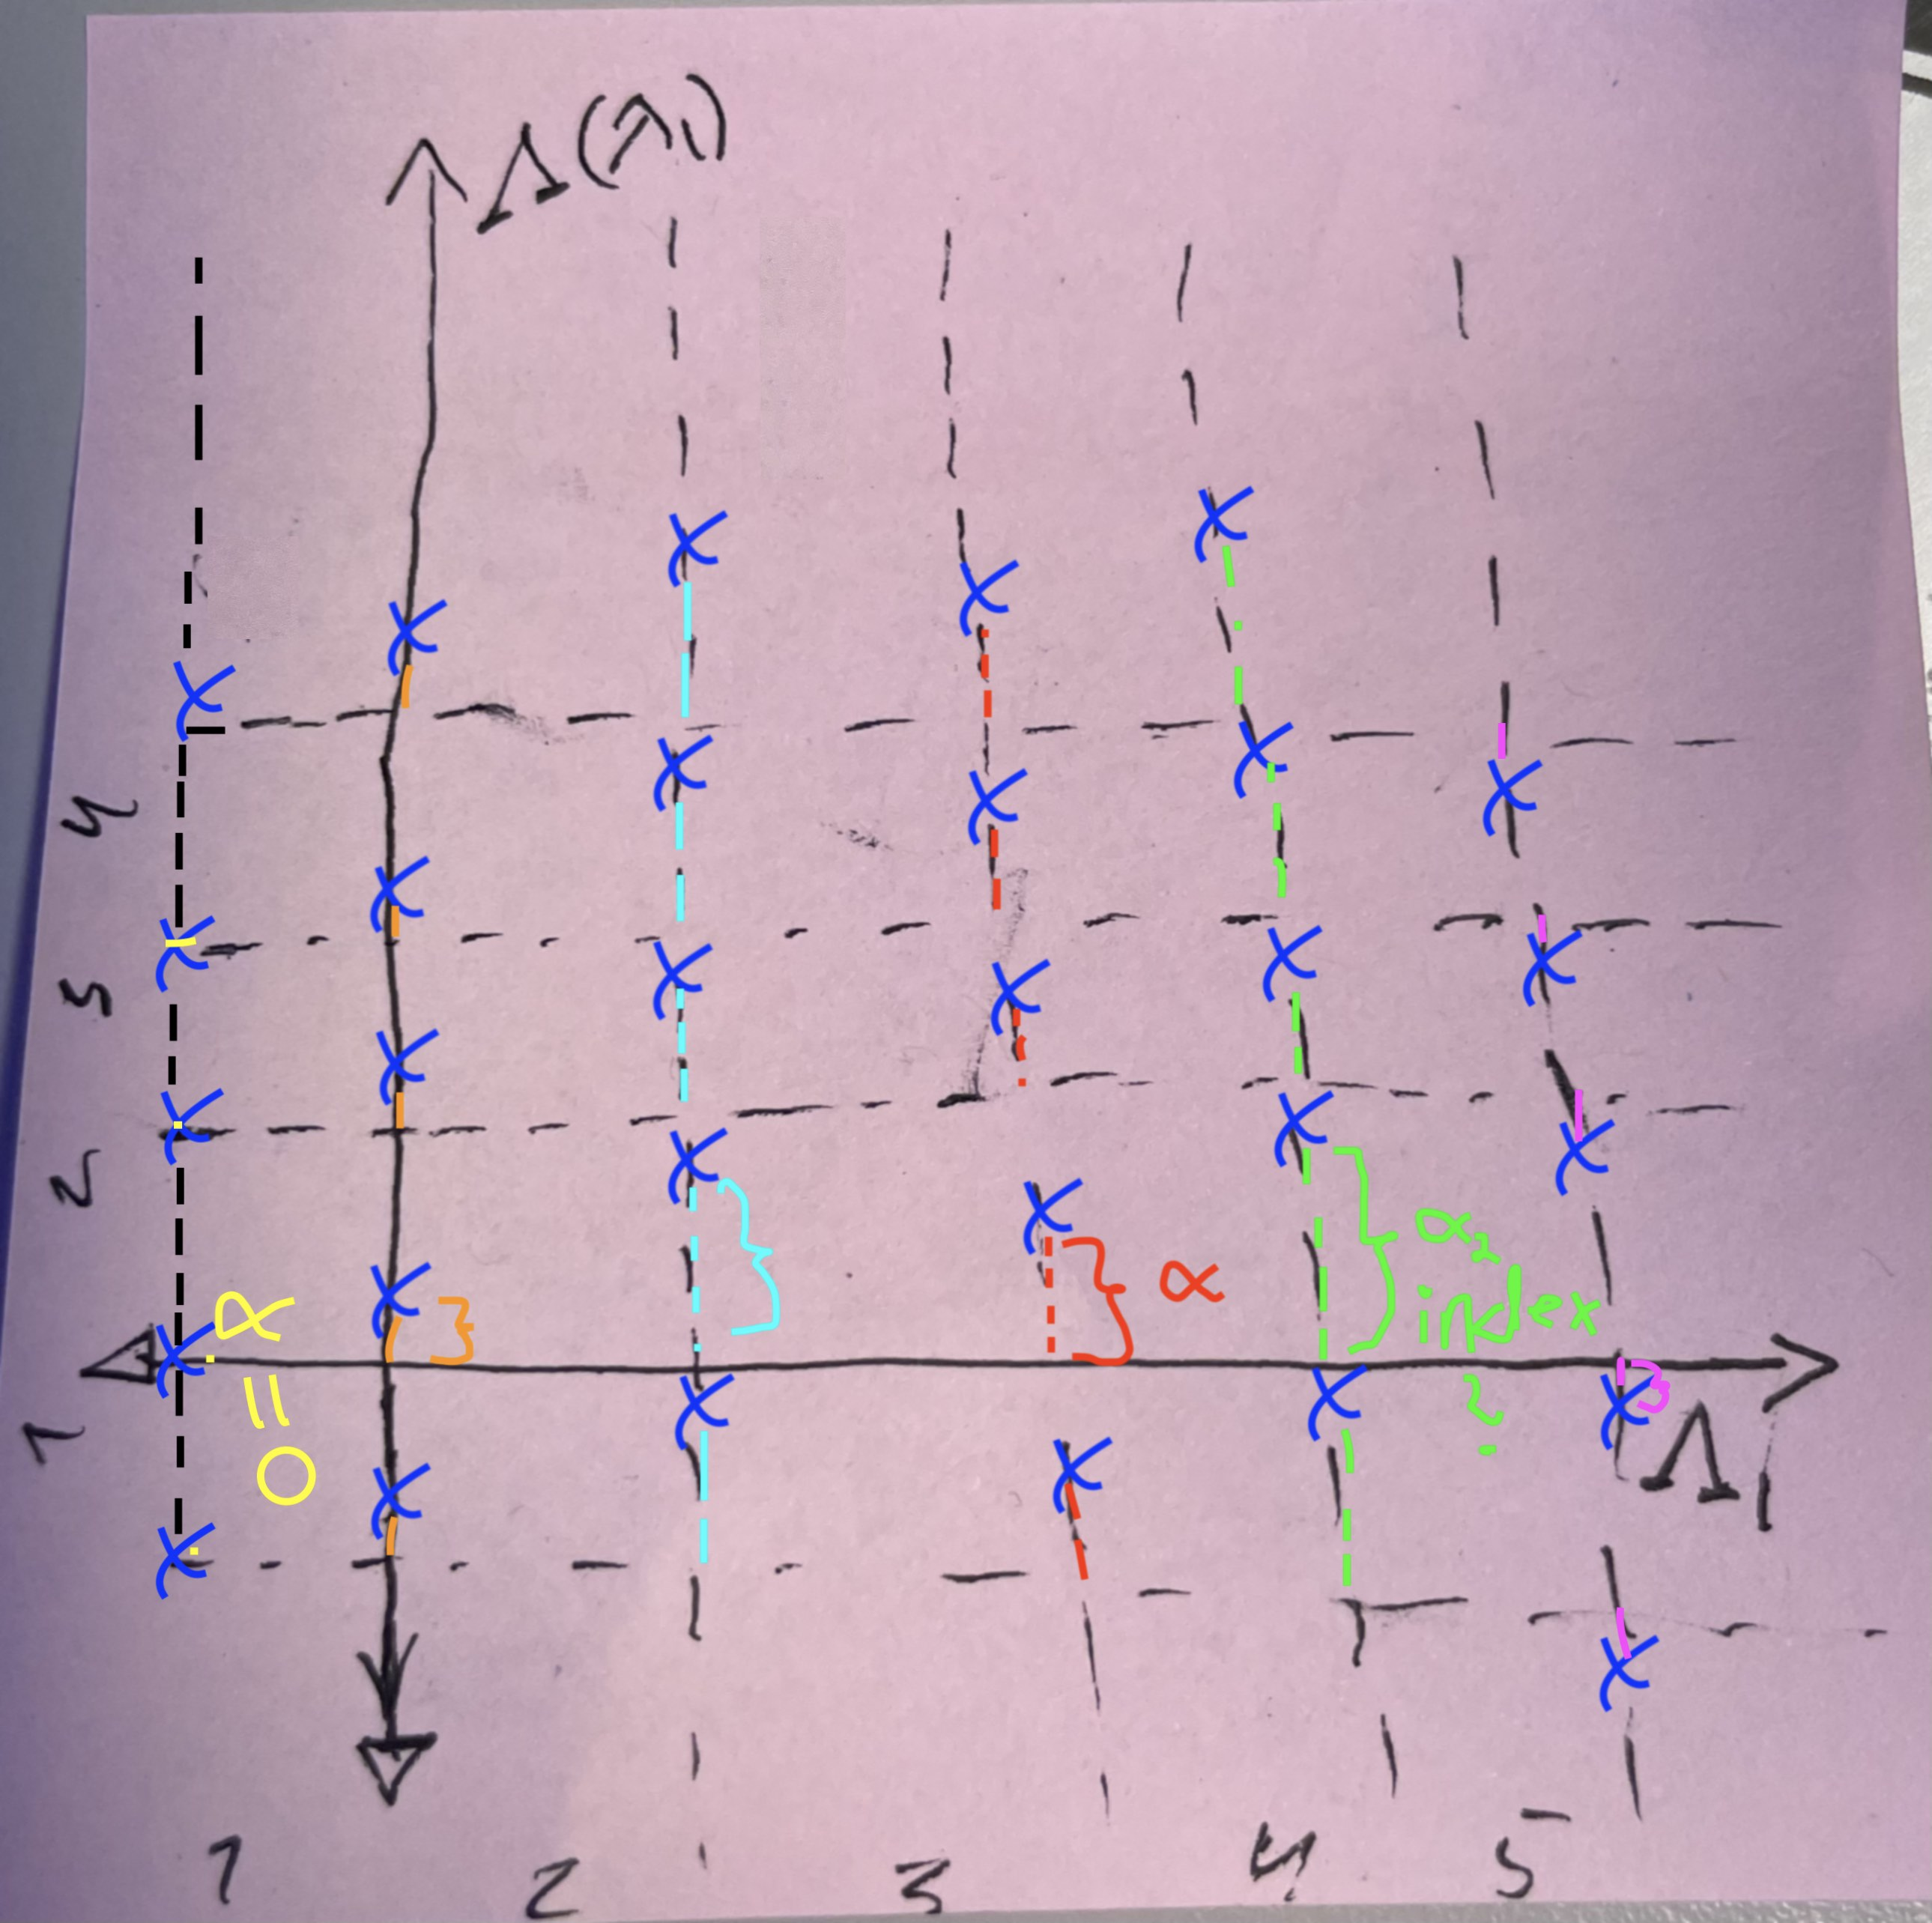
\includegraphics[width=0.9\linewidth]{multiple_shift_left_zero.jpg}
        %* Figure 3
        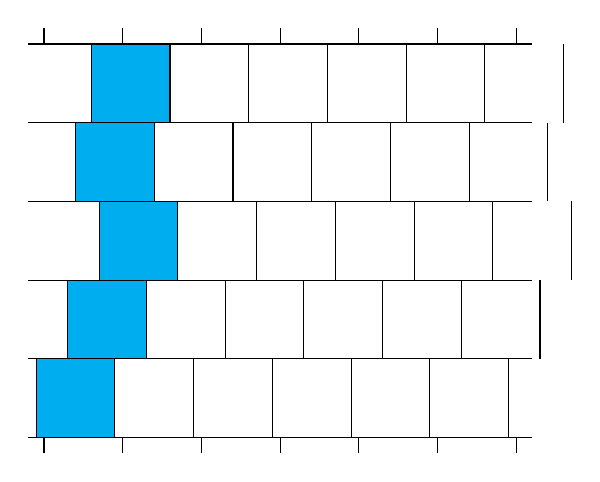
\begin{tikzpicture}[scale=1]
            % Define the tile
            \def\tile{
            % Draw the unit square
            \draw[fill=white] (0,0) rectangle (1,1);
            }
            \def\tiletwo{
            %\draw[fill=gray!65] (0,0) rectangle (1,1);
            \draw[fill=cyan] (0,0) rectangle (1,1);
            }

            % Shift list
            \def\BetaMinOne{-0.1}
            \def\BetaZero{0.3}
            \def\BetaOne{0.7}
            \def\BetaTwo{0.4}
            \def\BetaThree{0.6}
            
            % Draw the tiling pattern
            \foreach \x in {0,1,2,3,4}{
                \foreach \y in {0,1,2,3,4}{
                    \ifnum\y=0
                        \pgfmathsetmacro{\shiftX}{\x + \BetaMinOne}
                        \pgfmathsetmacro{\shiftY}{\y}
                        \pgfmathsetmacro{\shiftSingle}{\BetaMinOne}
                    \fi
                    \ifnum\y=1
                        \pgfmathsetmacro{\shiftX}{\x + \BetaZero}
                        \pgfmathsetmacro{\shiftY}{\y}
                        \pgfmathsetmacro{\shiftSingle}{\BetaZero}
                    \fi
                    \ifnum\y=2
                        \pgfmathsetmacro{\shiftX}{\x + \BetaOne} 
                        \pgfmathsetmacro{\shiftY}{\y} 
                        \pgfmathsetmacro{\shiftSingle}{\BetaOne}
                    \fi
                    \ifnum\y=3
                        \pgfmathsetmacro{\shiftX}{\x + \BetaTwo}
                        \pgfmathsetmacro{\shiftY}{\y}
                        \pgfmathsetmacro{\shiftSingle}{\BetaTwo}
                    \fi
                    \ifnum\y=4
                        \pgfmathsetmacro{\shiftX}{\x + \BetaThree}
                        \pgfmathsetmacro{\shiftY}{\y}
                        \pgfmathsetmacro{\shiftSingle}{\BetaThree}
                    \fi
                    % Drawing the left half-cubes
                    \ifnum\x=0
                        \draw[white, fill=white](\x-0.2,\y) rectangle (\x+\shiftSingle,\y+1);
                    \fi
                    % Drawing the right half-cubes
                    \ifnum\x=4
                        \ifthenelse{\lengthtest{\shiftSingle pt > 0.2 pt}}{
                            \draw[white] (\x+2+\shiftSingle,\y+1) -- (\x+2+\shiftSingle,\y);  % Right line
                        }{
                            \draw[black] (\x+2+\shiftSingle,\y+1) -- (\x+2+\shiftSingle,\y);  % Right line
                        }
                        %\draw[black] (\x+1,\y) -- (\x,\y+2);  % Left line
                        %\draw[black] (\x+2+\shiftSingle,\y) -- (\x+2+\shiftSingle,\y+1);  % Top
                        %\draw[black] (\x+1+\shiftSingle,\y+1) -- (\x+1+\shiftSingle,\y);  % Bottom line
                    \fi
                    % Drawing the rest of the middle cubes
                    \begin{scope}[shift={(\shiftX,\shiftY)}]
                        \tile % Draw the tile
                    \end{scope}
                    % Drawing a new line of shifted colored cubes on top at the first row
                    \ifnum\x=0
                    \begin{scope}[shift={(\shiftX,\shiftY)}]
                        \tiletwo
                    \end{scope}
                    \fi
                }   
            }
            % get the outline grid 
            % small black lines at the left and right
            \foreach \y in {0,1,2,3,4,5}{
                %\draw (0-0.2,\y) -- (0,\y);  % Left
                %\draw (6,\y) -- (6+0.2,\y);  % Right
                \draw (0-0.2,\y) -- (6+0.2,\y);  % Right
            }
            
            % small black lines at the top and bottom
            \foreach \x in {0,1,2,3,4,5,6}{
                \draw (\x,0-0.2) -- (\x,0);  % Top
                \draw (\x,5) -- (\x,5+0.2);  % Bottom
            }
        \end{tikzpicture}
        %* —————————————————
        \caption{Multiple row shifts}
        \label{fig:multiple_shift_horizontal_tiling}
    \end{subfigure}\quad
    \begin{subfigure}{.47\textwidth}
        \centering
        %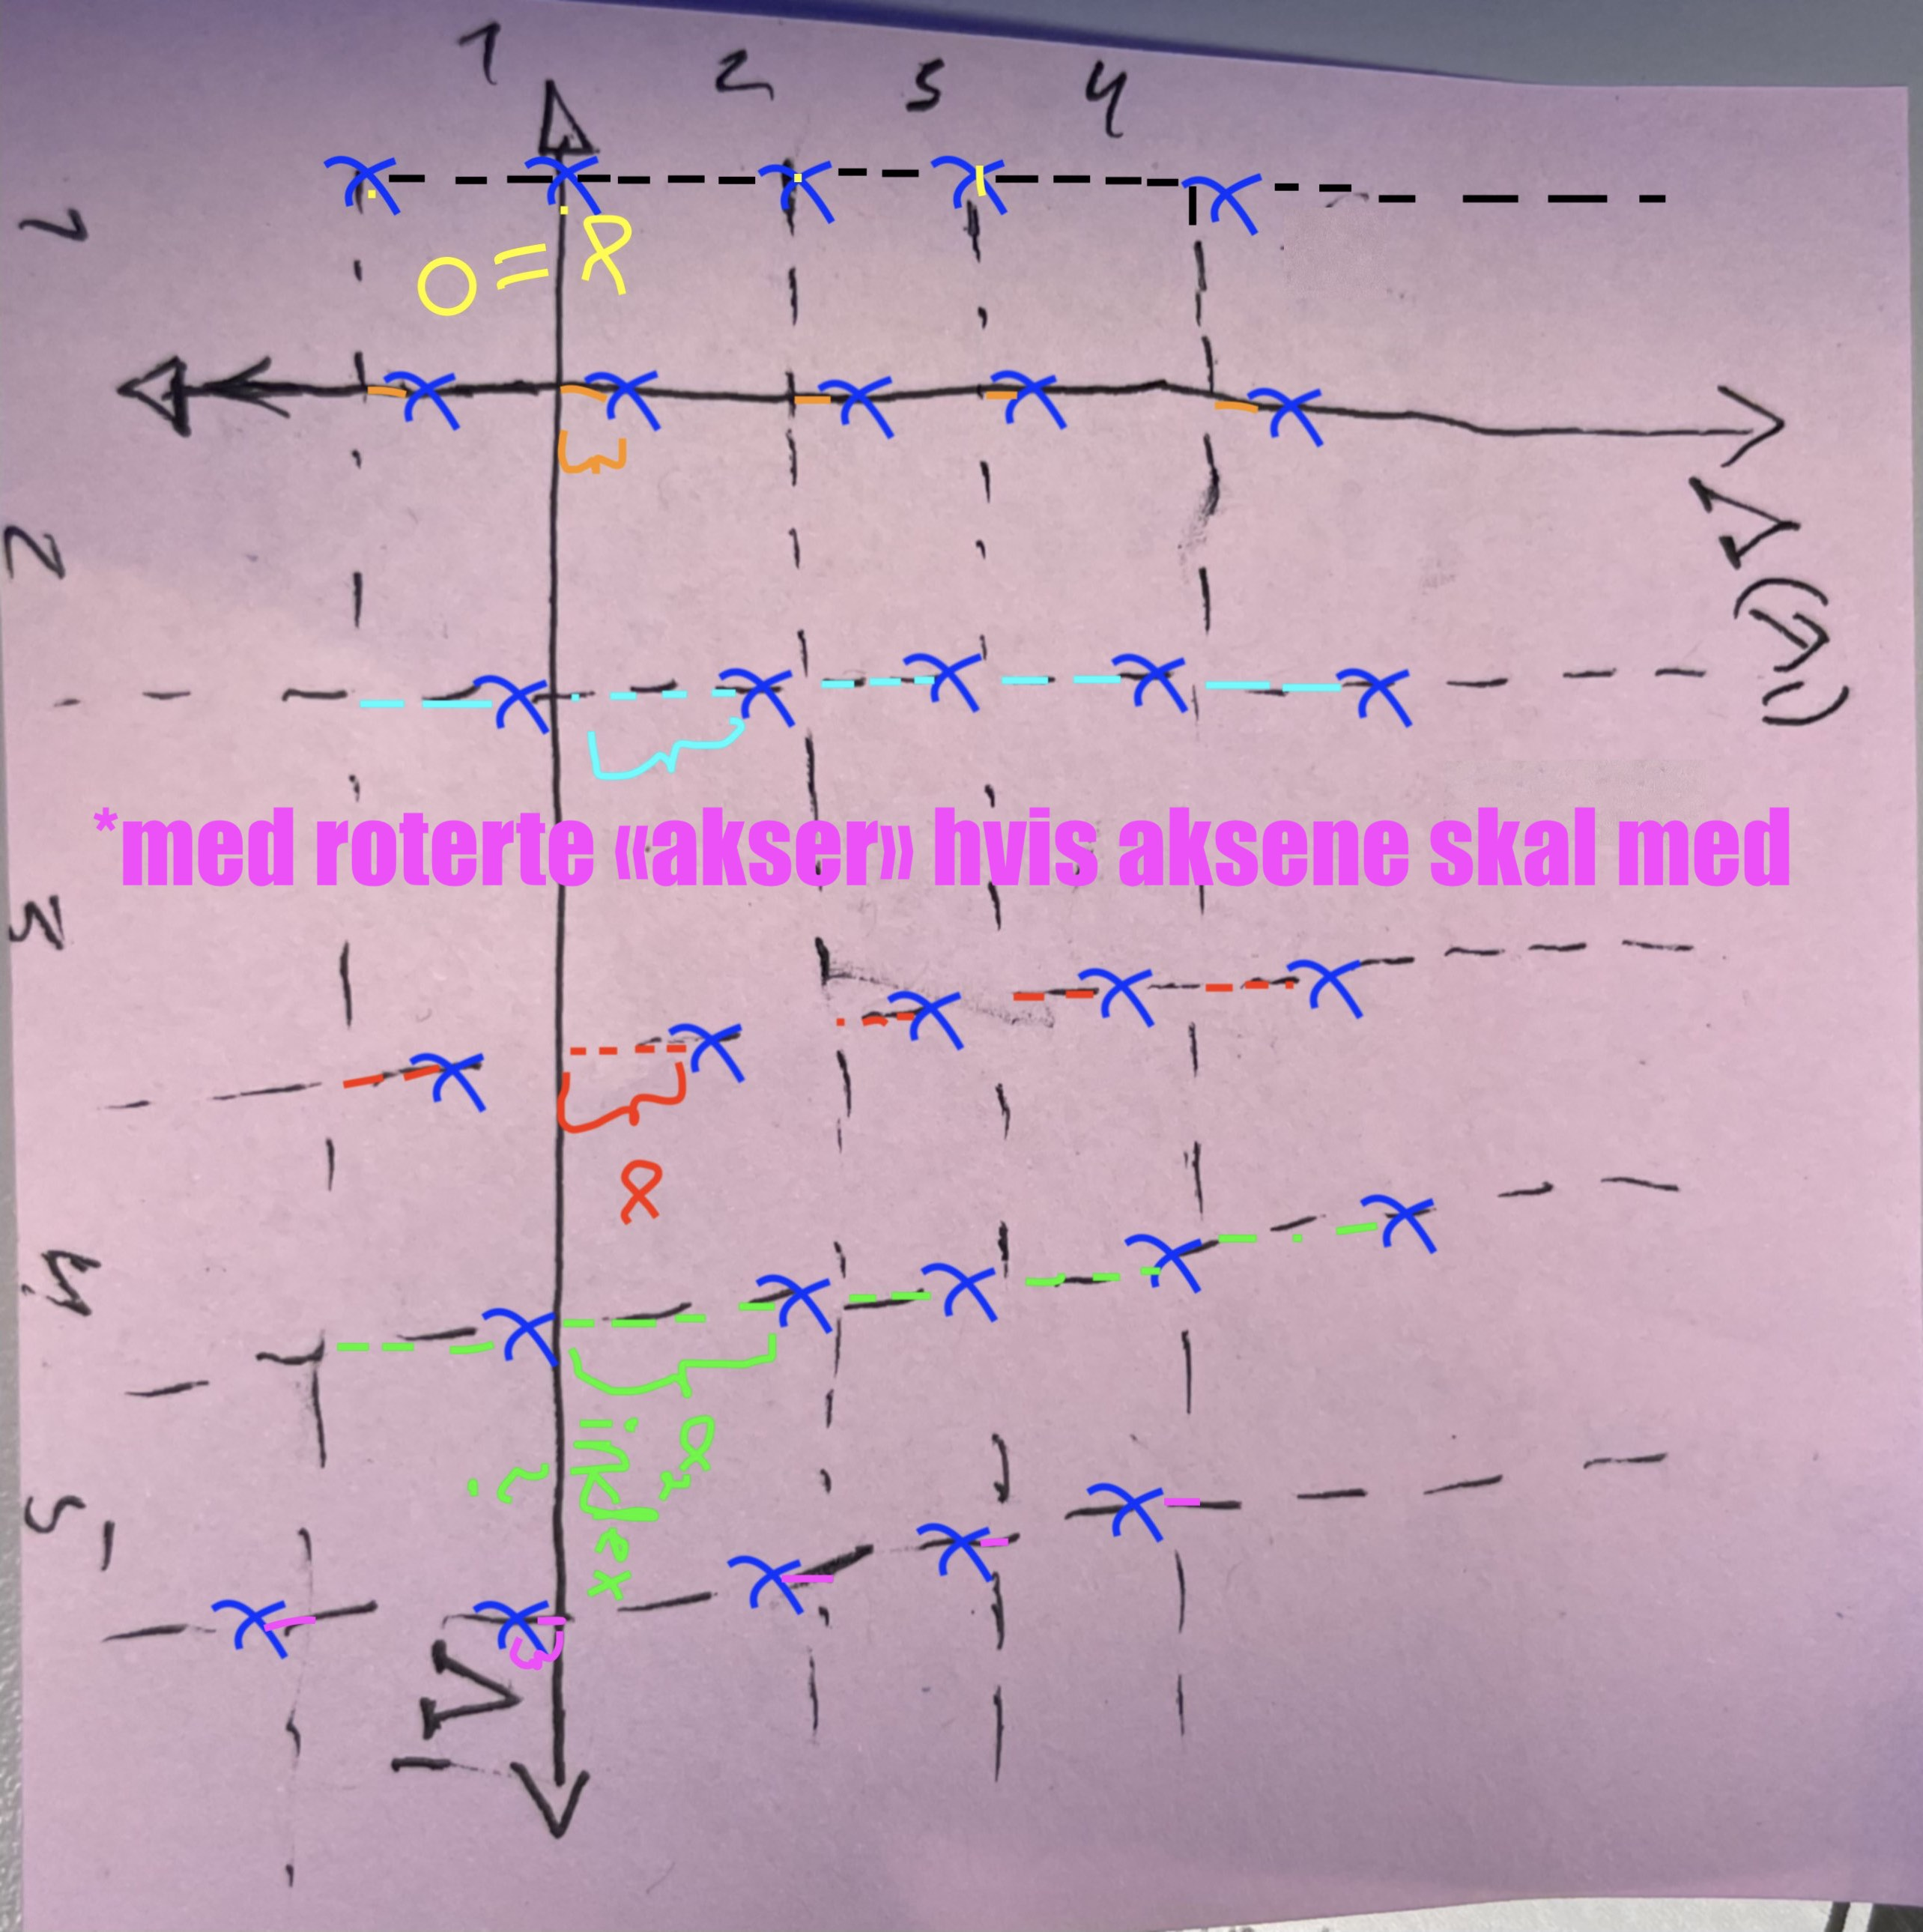
\includegraphics[width=0.9\linewidth]{multiple_shift_left_zero_horizontal.jpg}
        %* Figure 4
        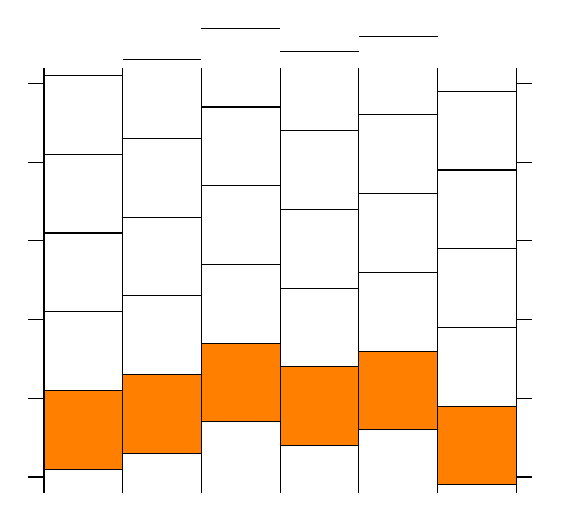
\begin{tikzpicture}[scale=1]
            % Define the tile
            \def\tile{
            % Draw the unit square
            \draw[fill=white] (0,0) rectangle (1,1);
            }
            \def\tiletwo{
            %\draw[fill=gray!65] (0,0) rectangle (1,1);
            \draw[fill=orange] (0,0) rectangle (1,1);
            %\draw[->] (0.5,0) -- (0.5,0.9);  % If arrows from the middle
            }

            % Shift list
            \def\BetaMinOne{0.1}
            \def\BetaZero{0.3}
            \def\BetaOne{0.7}
            \def\BetaTwo{0.4}
            \def\BetaThree{0.6}
            \def\BetaFour{-0.1}

            % Draw the tiling pattern
            \foreach \x in {0,1,2,3,4,5}{
                \foreach \y in {0,1,2,3}{
                    \ifnum\x=0
                        \pgfmathsetmacro{\shiftX}{\x}
                        \pgfmathsetmacro{\shiftY}{\y + \BetaMinOne}
                        \pgfmathsetmacro{\shiftSingle}{\BetaMinOne}
                    \fi
                    \ifnum\x=1
                        \pgfmathsetmacro{\shiftX}{\x}
                        \pgfmathsetmacro{\shiftY}{\y + \BetaZero}
                        \pgfmathsetmacro{\shiftSingle}{\BetaZero}
                    \fi
                    \ifnum\x=2
                        \pgfmathsetmacro{\shiftX}{\x} 
                        \pgfmathsetmacro{\shiftY}{\y + \BetaOne} 
                        \pgfmathsetmacro{\shiftSingle}{\BetaOne}
                    \fi
                    \ifnum\x=3
                        \pgfmathsetmacro{\shiftX}{\x}
                        \pgfmathsetmacro{\shiftY}{\y + \BetaTwo}
                        \pgfmathsetmacro{\shiftSingle}{\BetaTwo}
                    \fi
                    \ifnum\x=4
                        \pgfmathsetmacro{\shiftX}{\x}
                        \pgfmathsetmacro{\shiftY}{\y + \BetaThree}
                        \pgfmathsetmacro{\shiftSingle}{\BetaThree}
                    \fi
                    \ifnum\x=5
                        \pgfmathsetmacro{\shiftX}{\x}
                        \pgfmathsetmacro{\shiftY}{\y + \BetaFour}
                        \pgfmathsetmacro{\shiftSingle}{\BetaFour}
                    \fi
                    % Drawing the bottom half-cubes
                    \ifnum\y=0
                        \draw[white, fill=white](\x,\y-0.2) rectangle (\x+1,\y+\shiftSingle);
                    \fi
                    % Drawing the top half-cubes
                    \ifnum\y=3
                        \ifthenelse{\lengthtest{\shiftSingle pt > 0.2 pt}}{
                            \draw[white] (\x,\y+2+\shiftSingle) -- (\x+1,\y+2+\shiftSingle);  % Top
                        }{
                        \draw[black] (\x,\y+2+\shiftSingle) -- (\x+1,\y+2+\shiftSingle);  % Top
                        }
                        \draw[black] (\x,\y+1) -- (\x,\y+2);  % Left line
                        \draw[black] (\x+1,\y+2) -- (\x+1,\y+1);  % Right line
                        \draw[black] (\x+1,\y+1+\shiftSingle) -- (\x,\y+1+\shiftSingle);  % Bottom line
                        %\draw[red, fill=red](\x,\y+1) rectangle (\x+1,\y+2);
                    \fi
                    % Drawing the rest of the middle cubes
                    \begin{scope}[shift={(\shiftX,\shiftY)}]
                        \tile
                    \end{scope}
                    % Drawing a new line of shifted colored cubes on top at the first row
                    \ifnum\y=0
                        \begin{scope}[shift={(\shiftX,\shiftY)}]
                            \tiletwo
                        \end{scope}
                    \fi
                }  
            }
            % get the outline grid 
            % small black lines at the left and right
            \foreach \y in {0,1,2,3,4,5}{
                \draw (0-0.2,\y) -- (0,\y);  % Left
                \draw (6,\y) -- (6+0.2,\y);  % Right
            }
            % small black lines at the top and bottom
            \foreach \x in {0,1,2,3,4,5,6}{
                %\draw (\x,0-0.2) -- (\x,0);  % Top
                %\draw (\x,5) -- (\x,5+0.2);  % Bottom
                \draw (\x,0-0.2) -- (\x,5+0.2);  % Shift only in the vertical direction, therefore only one line
            }
        \end{tikzpicture}
        %* —————————————————
        \caption{Multiple column shifts}
        \label{fig:multiple_shift_vertical_tiling}
    \end{subfigure}
    \caption{Illustration of four tiling pairs for $\brac{I^2,\Lambda}$ covering $\R^2$. The cyan and orange colors represent shifts in the horizontal and vertical direction, respectively. The dashed line pattern in \cref{fig:single_shift_horizontal_tiling,fig:single_shift_vertical_tiling} highlights the single row or column which is shifted, and the filled cubes in \cref{fig:multiple_shift_horizontal_tiling,fig:multiple_shift_vertical_tiling} highlights the different shifts used for each row or column. Note that if this were a lattice tiling, all the cyan-filled or orange-filled squares would be on the same vertical or horizontal line, respectively.}
    \label{fig:tiling_figures}
\end{figure}

%\extractcolorspecs{Cyan}{\myColorModel}{\myColor} orange is \myColor\ in model %\myColorModel


%\section{Proof of Keller's \namecref{thrm:keller_tiling}}


%* Ikke si så veldig mye, 
%* Når vi kommer opp i d=2, så har vi åpenbart mer fleksibilitet, selv om Kellers theorem fortsatt er sant. Sånn at vi har jo den begrensningen om at vi må møtes i et heltall. 
%* Vise flexen og referere til kellers - Nei — Ikke begrunne det med Keller, 
%* I to dimensjoner har vi åpenbart større fleksibilitet fordi vi ikke trenger å ha Lattice tiling. Det kan vi vise ved eksempel. Dette ser vi i figur sånn og sånn, men det som også kommer frem så oppfyller jo Alle Kellers theorem, og det vil de også måtte gjøre. Det ville jeg kommentert, uten å, liksom, begrunne det til noe som helst.
%* Dette for å si noe om det (fleksibiliteten vi skal fange) allerede her
%* Vi skal se senere, (kap 5), det vi har tegnet her, strenkt tatt fanger all den fleksibiliteten vi har. Du har ikke noe mer fleksibilitet enn det du har skissert her. Du kan skyve på kolonnene, og du kan skyve på radene. Men det kommer vi tilbake til den og den seksjonen. Prøvd å skiserre. Da viser den figuren her egentlig all den fleksibiliteten vi har, men ikke sagt at du skal skal forklare noe mer om det nå. 


%* Prove the equivalence in chapter five. Here only show. 
%* Chapter 5, the part I showed in the spectra, also classifies all tiling sets.


\end{document}


